%
% This document is free; you can redistribute it and/or modify
% it under the terms of the GNU General Public License as published by
% the Free Software Foundation; either version 2 of the License, or
% (at your option) any later version.
%
% This document is distributed in the hope that it will be useful, but
% WITHOUT ANY WARRANTY; without even the implied warranty of
% MERCHANTABILITY or FITNESS FOR A PARTICULAR PURPOSE.  See the GNU
% General Public License for more details.
%
% You should have received a copy of the GNU General Public License
% along with this document; if not, write to the Free Software
% Foundation, Inc., 51 Franklin Street, Fifth Floor, Boston, MA
% 02110-1301, USA.
%
% Author: Bertoli Marco
%
\documentclass[10pt, twoside, a4paper]{book}
\usepackage{fancyhdr}
\usepackage{amsmath,amsfonts,amssymb}
\usepackage{graphicx}
\usepackage[english]{babel}
\usepackage{syntonly}
\usepackage{longtable}
\usepackage{inputenc}
\usepackage{tabularx}
\usepackage{inputenc}
\usepackage{listings}
\usepackage[dvipdfm]{hyperref}
\usepackage{tocbibind}
\hypersetup{ pdftitle={Java Modelling Tools users manual},
pdfauthor={Marco Bertoli}, bookmarksopen=true, bookmarksnumbered,
pdfstartview={FitH}, urlcolor=cyan, citebordercolor=000,
linkbordercolor=000, pdfhighlight=/n, }


% Change default margins
\topmargin -0.5 true in
\setlength{\evensidemargin}{1cm}
\setlength{\hoffset}{-1.5cm}
\setlength{\textwidth}{16.95cm}
\setlength{\textheight}{25cm}
% Space between figure and caption
\setlength{\abovecaptionskip}{-.3cm}

% Define itemize with less margin
\newenvironment{itemize*}
  {\begin{itemize}
    \setlength{\itemsep}{2pt}
    \setlength{\parskip}{0pt}}
  {\end{itemize}}

% Define enumerate with less margin
\newenvironment{enumerate*}
  {\begin{enumerate}
    \setlength{\itemsep}{2pt}
    \setlength{\parskip}{0pt}}
  {\end{enumerate}}

% Define description with less margin
\newenvironment{description*}
  {\begin{description}
    \setlength{\itemsep}{2pt}
    \setlength{\parskip}{0pt}}
  {\end{description}}

\author{Marco Bertoli}

\title{Java Modelling Tools users manual}

\begin{document}
\pagestyle{headings} \pagenumbering{roman} \setcounter{page}{-1}

% Title page
\begin{titlepage}
\begin{figure}[h]
\begin{center}

\includegraphics{img/poli}\\
Performance Evaluation Lab\\
Dipartimento di Elettronica e Informazione\\
Politecnico di Milano - Italy
\end{center}
\end{figure}
\newlength{\centeroffset}
\setlength{\centeroffset}{-0.5\oddsidemargin}
\addtolength{\centeroffset}{0.5\evensidemargin}

 \vspace*{\stretch{1}}
\noindent\hspace*{\centeroffset}\makebox[0pt][l]{\begin{minipage}{\textwidth}
\flushright {\Huge\bfseries Java Modelling Tools}\\
\noindent\rule[-1ex]{9.3cm}{5pt}\\[2.5ex]
\hfill\emph{\Huge users manual}
\end{minipage}}

\vspace{\stretch{0.1}}
\noindent\hspace*{\centeroffset}\makebox[0pt][l]{\begin{minipage}{\textwidth}
\flushright Version~0.3, \today
\end{minipage}}


\vspace{\stretch{2}}


\pagebreak
\begin{small}
  Copyright \copyright 2006 Performance Evaluation Lab - Dipartimento
  di Elettronica e Informazione - Politecnico di Milano.
  All rights reserved.

  Java Modelling Tools is free; you can redistribute it and/or modify it
  under the terms of the GNU General Public License as published by
  the Free Software Foundation; either version 2 of the License, or
  (at your option) any later version.

  Java Modelling Tools is distributed in the hope that it will be useful, but
  WITHOUT ANY WARRANTY; without even the implied warranty of
  MERCHANTABILITY or FITNESS FOR A PARTICULAR PURPOSE\@.  See the GNU
  General Public License for more details.

  You should have received a copy of the GNU General Public License
  along with Java Modelling Tools; if not, write to the Free Software
  Foundation, Inc., 675 Mass Ave, Cambridge, MA 02139, USA.

\end{small}

\end{titlepage}
\cleardoublepage

\tableofcontents \cleardoublepage

\pagenumbering{arabic} \setcounter{page}{1}

% Imports manuals
\chapter{Introduction}
\emph{The Java Modelling Tools} (JMT) is a free open source suite
consisting of \emph{six} tools  for performance evaluation,
capacity planning, workload characterization, and modelling of
computer and communication systems. The suite implements several
state-of-the-art algorithms for the exact, asymptotic and
simulative analysis of queueing network models, either with or
without product-form solution. Models can be described either
through \emph{wizard} dialogs or with a \emph{graphical}
user-friendly interface. The workload analysis tool is based on
clustering techniques. The suite incorporates an XML data layer
that enables full reusability of the computational engines.

The JMT suite is composed by the following tools: %GC

\medskip \noindent 
\includegraphics[scale=.5]{img/JSIMIcon}
\textbf{JSIM\emph{wiz}:} a wizard-based interface for the
discrete-event simulator JSIM for the analysis of queueing network
models. A sequence of \emph{wizard} windows helps in the
definition of the network properties. The JSIM simulation engine
supports several probability distributions for characterizing
service and inter-arrival times. Load-dependent strategies using
arbitrary functions of the current queue-length can be specified.
JSIM\emph{wiz} supports state-independent routing strategies,
e.g., Markovian or round robin, as well as state-dependent
strategies, e.g., routing to the server with minimum utilization,
or with the shortest response time, or with minimum queue-length.
The simulation engine supports several extended features not
allowed in product-form models, namely, finite capacity regions
(i.e., blocking), fork-join servers (i.e., parallelism), and
priority classes. The JSIM performs automatically the transient
detection, based on spectral analysis, computes and plots on-line
the estimated values within the confidence intervals. What-if analyses, where
a sequence of simulations is run for different values of control
parameters, are also supported.

\medskip \noindent 
\includegraphics[scale=.5]{img/JMODELIcon}
\textbf{JSIM\emph{graph}:} a \emph{graphical} user-friendly
interface for the same simulator engine JSIM used by
JSIM\emph{wiz}. It integrates the same functionalities of
JSIM\emph{wiz} with an intuitive graphical workspace. This allows
an easy description of network structure, as well as a simplified
definition of the input and execution parameters. Network
topologies can be exported in vectorial or raster image formats.

\medskip \noindent 
\includegraphics[scale=.5]{img/JMVAIcon}
\textbf{JMVA:} for the \emph{exact} analysis of single-class or
multiclass product-form queueing networks, processing \emph{open,
closed} or \emph{mixed} workloads. A stabilized version of the
Mean Value Analysis MVA algorithm is used. Network structure is
specified by textual \emph{wizards}. What-if analyses and
graphical representation of the results are provided.

\medskip \noindent 
\includegraphics[scale=.5]{img/JMCHIcon}
\textbf{JMCH:} it applies a simulation technique to solve a single
station model, with finite (M/M/1/k) or infinite queue (M/M/1),
and shows the underlying Markov Chain. It is possible to
dynamically change the arrival rate and service time of the
system.

\medskip \noindent 
\includegraphics[scale=.5]{img/JABAIcon}
\textbf{JABA:} for the identification of \emph{bottlenecks} in
multiclass closed product-form networks using efficient convex
hull algorithms. Up to three customer classes are supported. It is
possible to identify potential bottlenecks corresponding to the
different mixes of customer classes in execution. Models with
thousands of queues can be analyzed efficiently.
\emph{Optimization} studies (e.g., throughput maximization,
minimization of response time, identification of the optimal load)
can be performed through the identification of the
\emph{saturation sectors}, i.e., the mixes of customer classes in
execution that saturate more than one resource simultaneously.

\medskip \noindent 
\includegraphics[scale=.5]{img/JWATIcon}
\textbf{JWAT:} supports the \emph{workload characterization}
process. Some standard formats for input file are provided (e.g.,
Apache HTTP and IIS log files), customized formats may also be
specified. The imported data can initially be analyzed using
descriptive statistical techniques (e.g, means, correlations,
histograms, boxplots, scatterplots), either for univariate or
multivariate data. Algorithms for data scaling, sample extraction,
outlier filtering, k-means and fuzzy k-means clustering for
identifying similarities in the input data are provided. These
techniques allow the identification of cluster of customers having
similar characteristics. The clusters centroids represent the mean
values of the parameters of the classes (e.g., CPU time, n.o of
I/Os, n.o of web pages pages accessed) that can be used for the
workload parameterization. 

\section{Starting with the JMT suite}
Double click on the JMT icon

\includegraphics[scale=.5]{img/JMTIcon} on your \emph{program group} or
on the \emph{desktop}, or open the \emph{command prompt} and type
from the installation directory:
\begin{verbatim}
    java -jar JMT.jar
\end{verbatim}
The window of \autoref{fig:startscreen} will be shown.

\begin{figure}[htbp]
    \begin{center}
        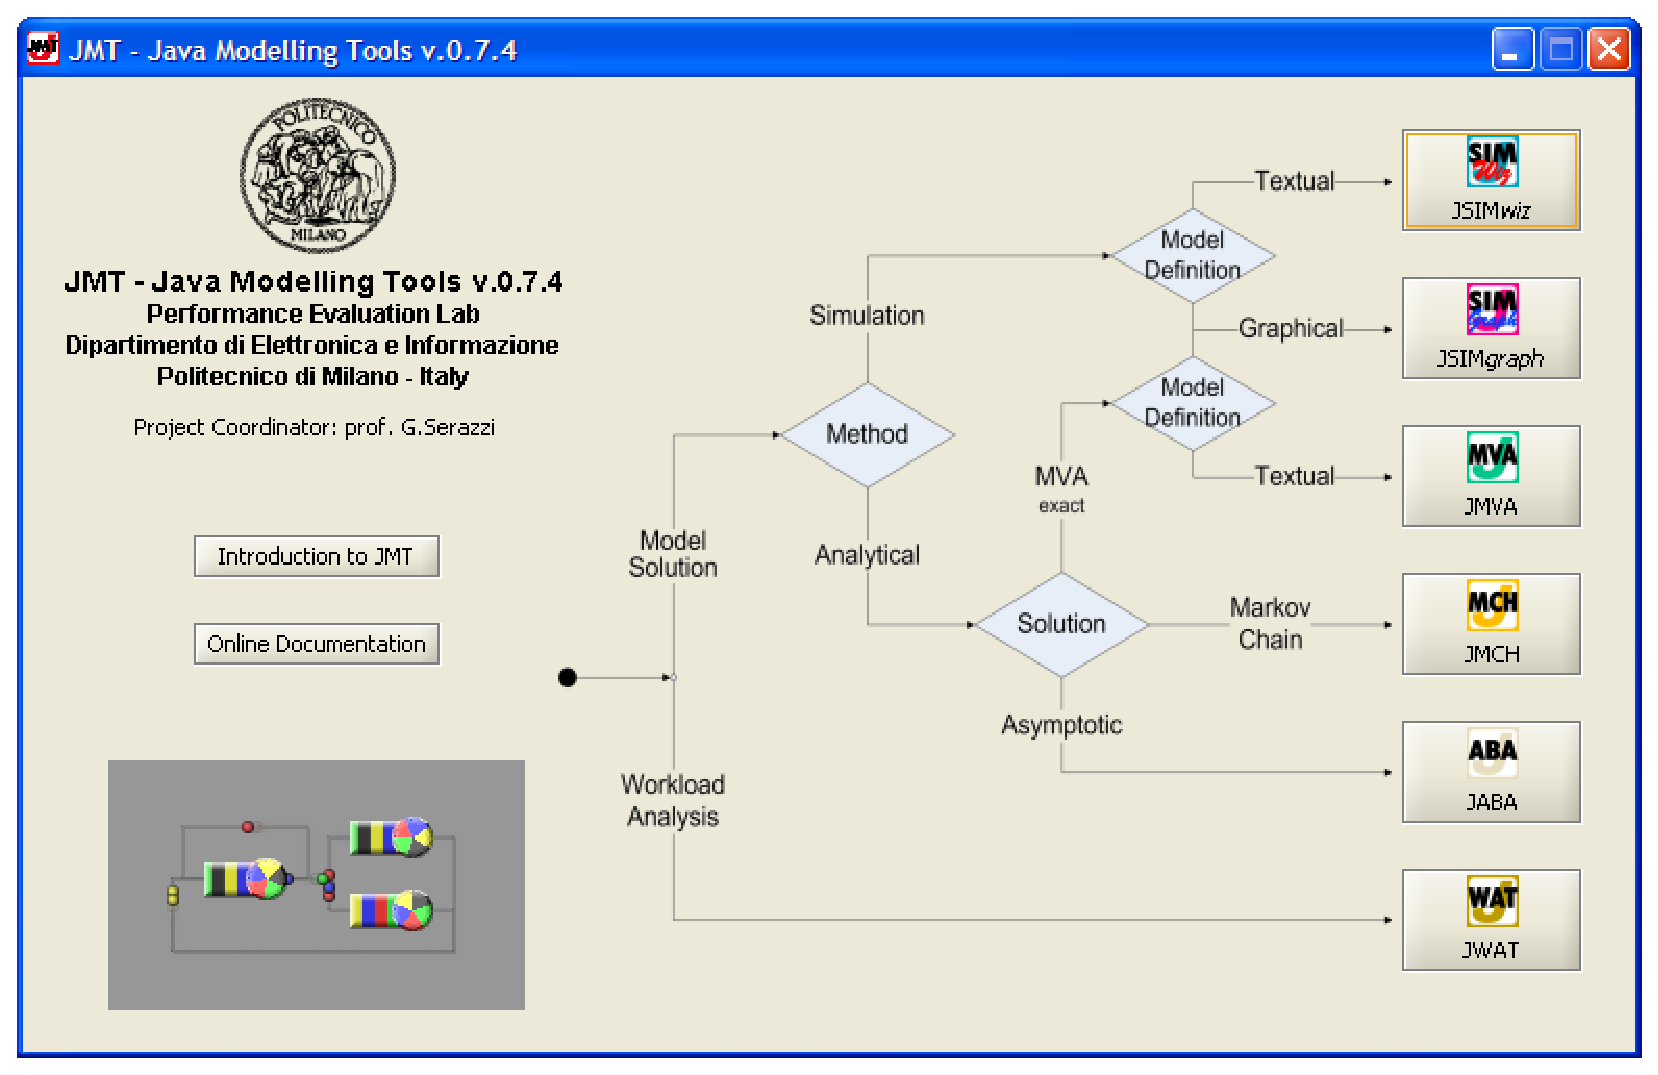
\includegraphics[scale=.5]{img/StartScreen}
    \end{center}
    \caption{The JMT suite Starting Screen}
    \label{fig:startscreen}
\end{figure}

This starting screen is used to select the application of the
suite to be executed by clicking on the corresponding button. The
flow chart should help the user to select the application that
best fits its needs.

In the following chapters the tools will be examined in details
and some examples are given. This manual is intended for the
general user that wants to learn how to interact with JMT.
Advanced users that want to learn details on internal data
structures, computational engines and XML interfaces should refer
to \emph{JMT system manual}.\\
Several other documents related to JMT description and
applications are provided with the suite. Click on \texttt{Online
Documentation} button to access the library. An exercise
book is also available.\\

%
% This document is free; you can redistribute it and/or modify
% it under the terms of the GNU General Public License as published by
% the Free Software Foundation; either version 2 of the License, or
% (at your option) any later version.
%
% This document is distributed in the hope that it will be useful, but
% WITHOUT ANY WARRANTY; without even the implied warranty of
% MERCHANTABILITY or FITNESS FOR A PARTICULAR PURPOSE.  See the GNU
% General Public License for more details.
%
% You should have received a copy of the GNU General Public License
% along with this document; if not, write to the Free Software
% Foundation, Inc., 51 Franklin Street, Fifth Floor, Boston, MA
% 02110-1301, USA.
%
% Author: Bertoli Marco
%
\chapter{JMVA}
\label{cha:jmva}
\section{Overview}
JMVA solves open, closed and mixed product form \cite{BCMP} queueing
networks with the exact MVA algorithm \cite{MVA}. In order to avoid
fluctuations of the solutions when the model contains load dependent
stations, the implemented algorithm is a stabilized version
\cite{AMVA} of the classic MVA algorithm.

Resources may be of two types: \emph{queueing} (either with
\texttt{load independent} or \texttt{load dependent} service times)
and \texttt{delay}. The model is described in alphanumeric way: user
is guided through the definition process by steps of a \emph{wizard}
interface (5 or 6 steps). What-if analyses, where a sequence of model are solved for different
values of parameters, are also possible (see \autoref{sec:jmva:whatif}). A graphical interface to describe the model in a user-friendly environment is also available, see \autoref{cha:jmodel} for details.

\subsection{Starting the alphanumeric MVA solver}
Selecting 
\includegraphics[scale=.5]{img/JMVAIcon} button on the
starting screen, \autoref{fig:jmva:Classes} window shows up.
\begin{figure}[htbp]
    \begin{center}
        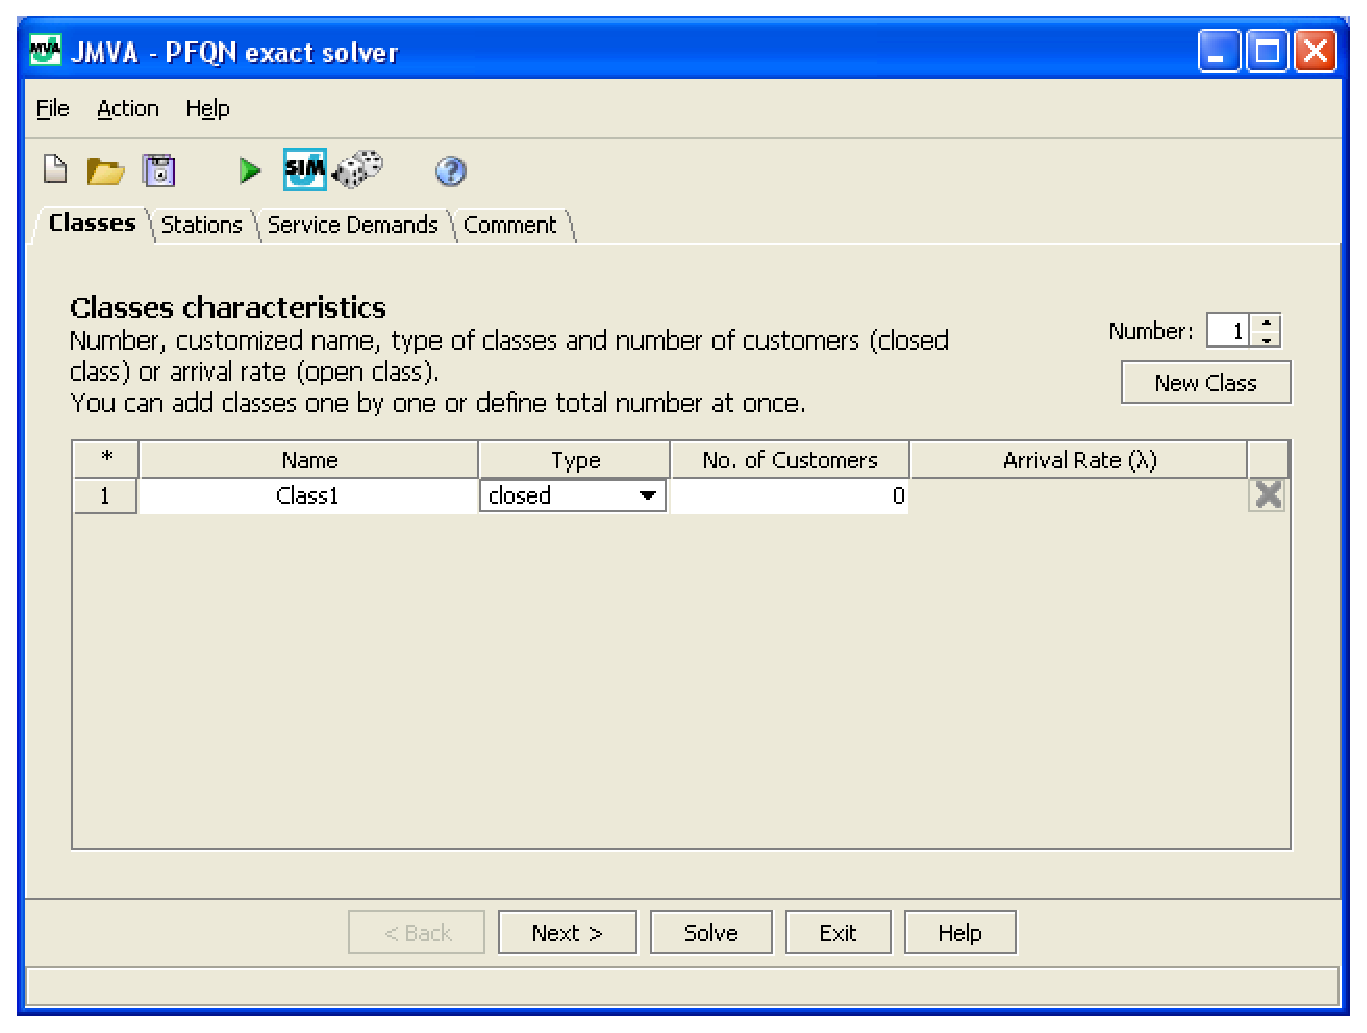
\includegraphics[scale=.5]{img/jmva/classes}
    \end{center}
    \caption{Classes tab}
    \label{fig:jmva:Classes}
\end{figure}
Three main areas are shown:
\begin{description}
\item[Menu :] it is organized into three groups of functions. To use a
menu, click on the menu heading and choose the appropriate option.
For the description of menu entries, see \autoref{sec:jmva:Menu}
\item[Toolbar :] contains some buttons to speed up access to JMVA functions
(e.g. New model, Open, Save\dots See \autoref{sec:jmva:Menu} for
details). If you move the mouse pointer over a button a tooltip will
be shown up.
\item[Page Area :] this is the core of the window. All MVA parameters are grouped in
different tabs. You can modify only a subset of them by selecting
the right tab, as will be shown later.
\end{description}

\section{Model definition}
Models with one or multiple customer classes provide estimates of
performance measures. For a brief description of basic terminology
please refer to \autoref{cha:glossary}.

In the case of single class models, the workload is characterized by
two inputs: the set of service demands, one for each resource, and
the workload intensity. On the other hand, in multiple class models,
a matrix of service demands is requested \cite{Lazowska}.

\subsection{Defining a new model}
To define a new model select toolbar button

\includegraphics[scale=.8]{img/jmva/new} or the \emph{New} command
from \emph{File} menu. The following parameters must be defined:
\begin{enumerate*}
\item \texttt{Classes} with their workload intensities (number of customer
$N$ for closed classes and arrival rate $\lambda$ for open classes)
\item \texttt{Stations} (service centers)
\item \texttt{Service demands} (or Service Times and Visits)
\item Optional short \texttt{Comment}
\end{enumerate*}

The execution of JMVA provides, for each class and each station, the
following performance indices:

\begin{itemize*}
\item Throughput
\item Queue Length
\item Residence Time
\item Utilization
\end{itemize*}

\noindent The following \emph{aggregate} indices are provided:
\begin{itemize*}
\item System Throughput
\item System Response Time
\item Average number of customers in the system
\end{itemize*}

\subsubsection{Input tabs}
As can be seen in \autoref{fig:jmva:Classes}, the parameters that
must be entered in order to define a new model are divided in four
tabs: \texttt{Classes}, \texttt{Stations}, \texttt{Service Demands}
and \texttt{Comment}.

Tabs number can become five, if you click  \emph{Service Times and
Visits} button in \texttt{Service Demands Tab}. As will be discussed
in \autoref{sec:jmva:ServiceDemand}, the \texttt{Service Demands
Tab} will be hidden and it will appear \texttt{Service Times Tab}
and \texttt{Visit Tab}. You can navigate through tabs:
\begin{itemize*}
\item using sequential wizard buttons, if enabled, at the bottom of
the window (\autoref{fig:jmva:Wizardbuttons})
\item using sequential buttons located in menu
\item using the tab selector, clicking on the corresponding
tab (\autoref{fig:jmva:Tabselector})
\end{itemize*}

\begin{figure}[htbp]
    \begin{center}
        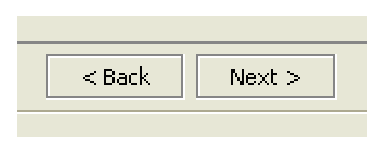
\includegraphics[scale=.5]{img/jmva/wizBut}
    \end{center}
    \caption{Wizard buttons}
    \label{fig:jmva:Wizardbuttons}
\end{figure}

\begin{figure}[htbp]
    \begin{center}
        
\includegraphics[scale=.5]{img/jmva/tabSel}
    \end{center}
    \caption{Tab selector}
    \label{fig:jmva:Tabselector}
\end{figure}

\subsection{Classes Tab}
An example screenshot of this tab can be seen in
\autoref{fig:jmva:Classes}. This tab allows to characterize customer
classes of the model. Your model will be a single class model if and
only if there will be only one class, closed or open. On the
contrary multiple class models will have at least two classes,
closed and/or open.

The number of classes in the model can be specified in the
corresponding input area, shown in \autoref{fig:jmva:ClassNum} and
can be modified using the keyboard or using the spin controls.

\begin{figure}[htbp]
    \begin{center}
        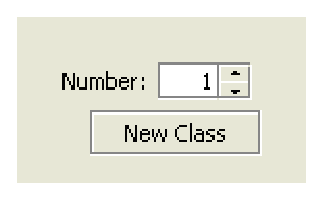
\includegraphics[scale=.5]{img/jmva/classNum}
    \end{center}
    \caption{Number of classes}
    \label{fig:jmva:ClassNum}
\end{figure}

Using the delete button

\includegraphics[scale=.6]{img/jmva/x} associated to a specific
class, a class can be removed provided that there will be at least
one class after the deletion. Similar result may be obtained using
spin controls, decreasing classes number; in this case last inserted
class will be removed.

Default class names are \emph{Class1}, \emph{Class2}, \dots
\emph{ClassN}. A model can be personalized by changing this names.

In \autoref{fig:jmva:3Classes} there are three classes of customers,
two closed and one open. The third class has the default name
\emph{Class3} while the other two classes have personalized names,
namely \emph{ClosedClass} and \emph{OpenClass}.

\begin{figure}[htbp]
    \begin{center}
        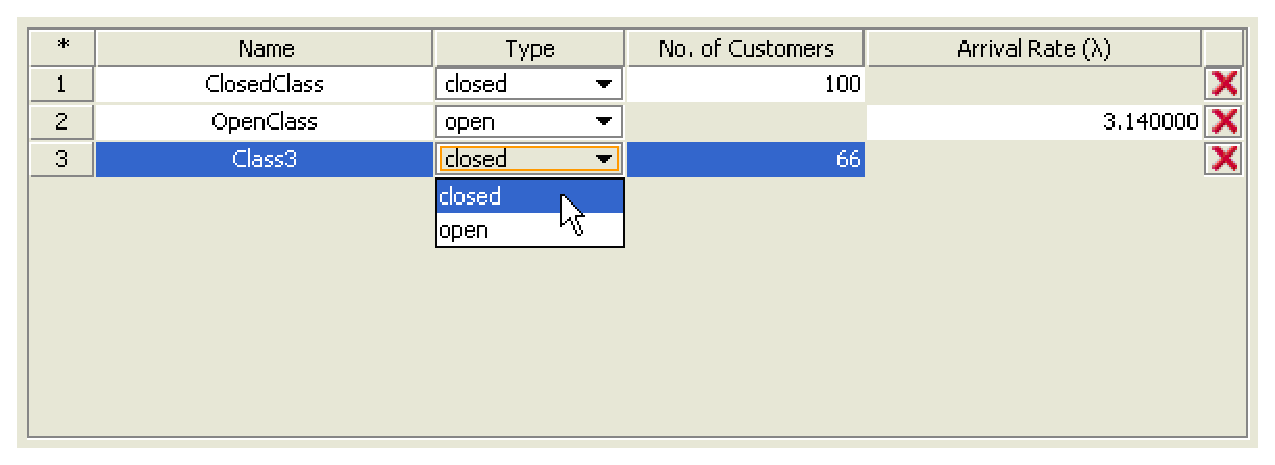
\includegraphics[scale=.5]{img/jmva/3classes}
    \end{center}
    \caption{Defining the classes types}
    \label{fig:jmva:3Classes}
\end{figure}

A class type can be \texttt{Open} or \texttt{Closed}. It is
important to define each class type because a closed class workload
is described by the number of customers in each class and the open
classes workload is described by the customer arrival rate for each
class.

As can be seen in \autoref{fig:jmva:3Classes}, a class type can be
selected in a combo-box. The input boxes \emph{No. of Customers
($N$)} referring to closed classes accept only positive integer
numbers; the input boxes of the \emph{Arrival Rate ($\lambda$)}
referring to open classes, accept positive real numbers
(\autoref{fig:jmva:workload}).

\begin{figure}[htbp]
    \begin{center}
        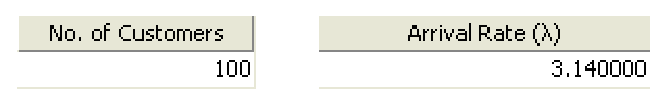
\includegraphics[scale=.5]{img/jmva/NL}
    \end{center}
    \caption{Workload definition of the number of customers of a closed
    class ($N=100$) and the arrival rate of an open class ($\lambda=3.14$)}
    \label{fig:jmva:workload}
\end{figure}

\subsection{Stations Tab}
The number of stations of the model can be specified in the
corresponding input area (\autoref{fig:jmva:stationNum}) and can be
modified using the keyboard or the spin controls.

\begin{figure}[htbp]
    \begin{center}
        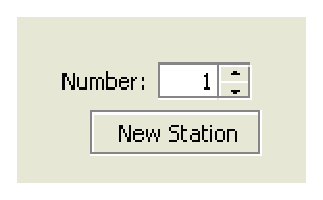
\includegraphics[scale=.5]{img/jmva/stationNum}
    \end{center}
    \caption{Number of stations}
    \label{fig:jmva:stationNum}
\end{figure}

Using the delete button

\includegraphics[scale=.6]{img/jmva/x} associated to a specific
station, a station can be removed provided that there will be at
least one station after the deletion. Similar result may be obtained
using spin controls, decreasing stations number; in this case last
inserted station will be removed.

Default station names are \emph{Station1}, \emph{Station2}, \dots
\emph{StationN}. In order to personalize your model, you can change
and give names other than default ones.

In \autoref{fig:jmva:stations} there is only one station with
default name \emph{Station4} and there are three stations with
personalized names: \emph{CPU}, \emph{Disk1} and \emph{Disk2}.

\begin{figure}[htbp]
    \begin{center}
        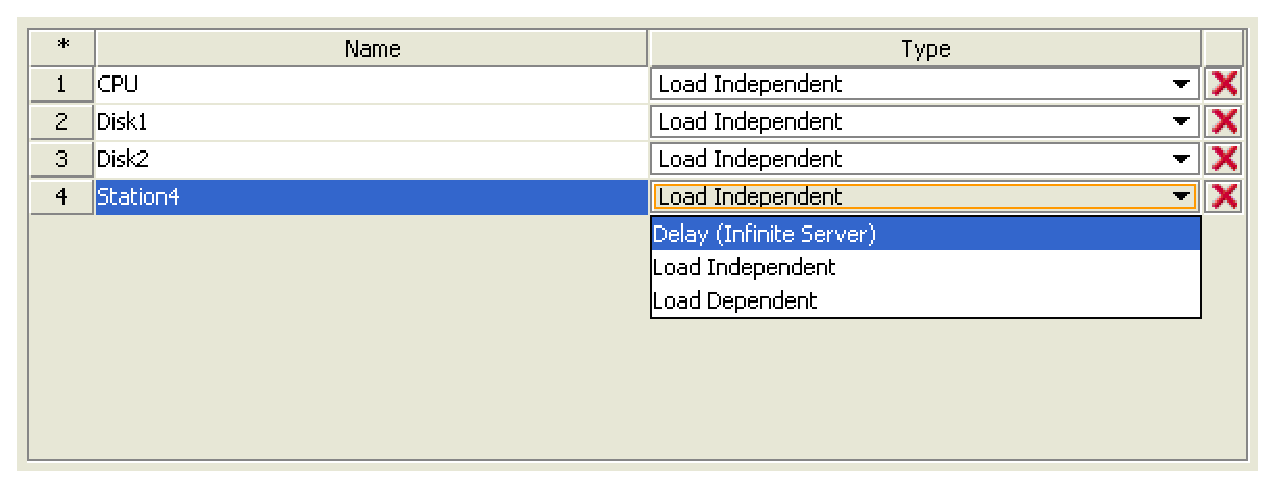
\includegraphics[scale=.5]{img/jmva/4stations}
    \end{center}
    \caption{Defining the stations type}
    \label{fig:jmva:stations}
\end{figure}

A station type can be \texttt{Load Independent}, \texttt{Load
Dependent} or \texttt{Delay}. You can insert in your model a
\texttt{Load Depend} center only if there is a unique closed
class\footnote{Multiclass, open and mixed models with load dependent
stations are not supported yet}; in all other cases the combo-box
will be disabled.

It is important to define each station type because if a station is
\texttt{Load Dependent} a set of service demand - or a set of
service times and the number of visit - must be defined (one service
demand/time for each possible value of queue length inside the
station).

In \autoref{sec:jmva:ServiceDemand} we will explain this concept
with more details.

\subsection{Service Demands, Service Times and Visits Tabs}
\label{sec:jmva:ServiceDemand} Service Demands can be defined in two
ways:
\begin{itemize*}
\item directly, by entering Service Demands ($D_{kc}$)
\item indirectly, by entering Service Times ($S_{kc}$) and Visits ($V_{kc}$)
\end{itemize*}

Service demand $D_{kc}$ is the total service requirement, that is
the average amount of time that a customer of class $c$ spends in
service at station $k$ during one interaction with the system, i.e.
it's complete execution. Service time $S_{kc}$ is the average time
spent by a customer of class $c$ at station $k$ for a single visit
at that station while $V_{kc}$ is the average number of visits at
that resource for each interaction with the system.

Remember that $D_{kc} = V_{kc} * S_{kc}$ so it's simple to compute
service demands matrix starting from service times and visits
matrixes. Inverse calculation is performed with the following
algorithm:
\[
V_{kj} = \left\{
\begin{array}{ccl} 1 & \textrm{if} & D_{kc} > 0 \\
0 & \textrm{if} & D_{kc} = 0 \end{array}\right.
\]
\[
S_{kc} = \left\{ \begin{array}{ccl} D_{kc} & \textrm{if} & D_{kc}
> 0 \\ 0 & \textrm{if} & D_{kc} = 0 \end{array}\right.
\]

\subsubsection{Service Demands Tab}
In this tab you can insert directly Service Demands $D_{kc}$ for
each pair \{station~$k$-class~$c$\} in the model. In
\autoref{fig:jmva:ServiceDemandsTab} a reference screenshot can be
seen: notice that a value for every $D_{kc}$ element of the
$D$-matrix has already been specified because default value assigned
to newly created stations is zero.

\begin{figure}[htbp]
    \begin{center}
        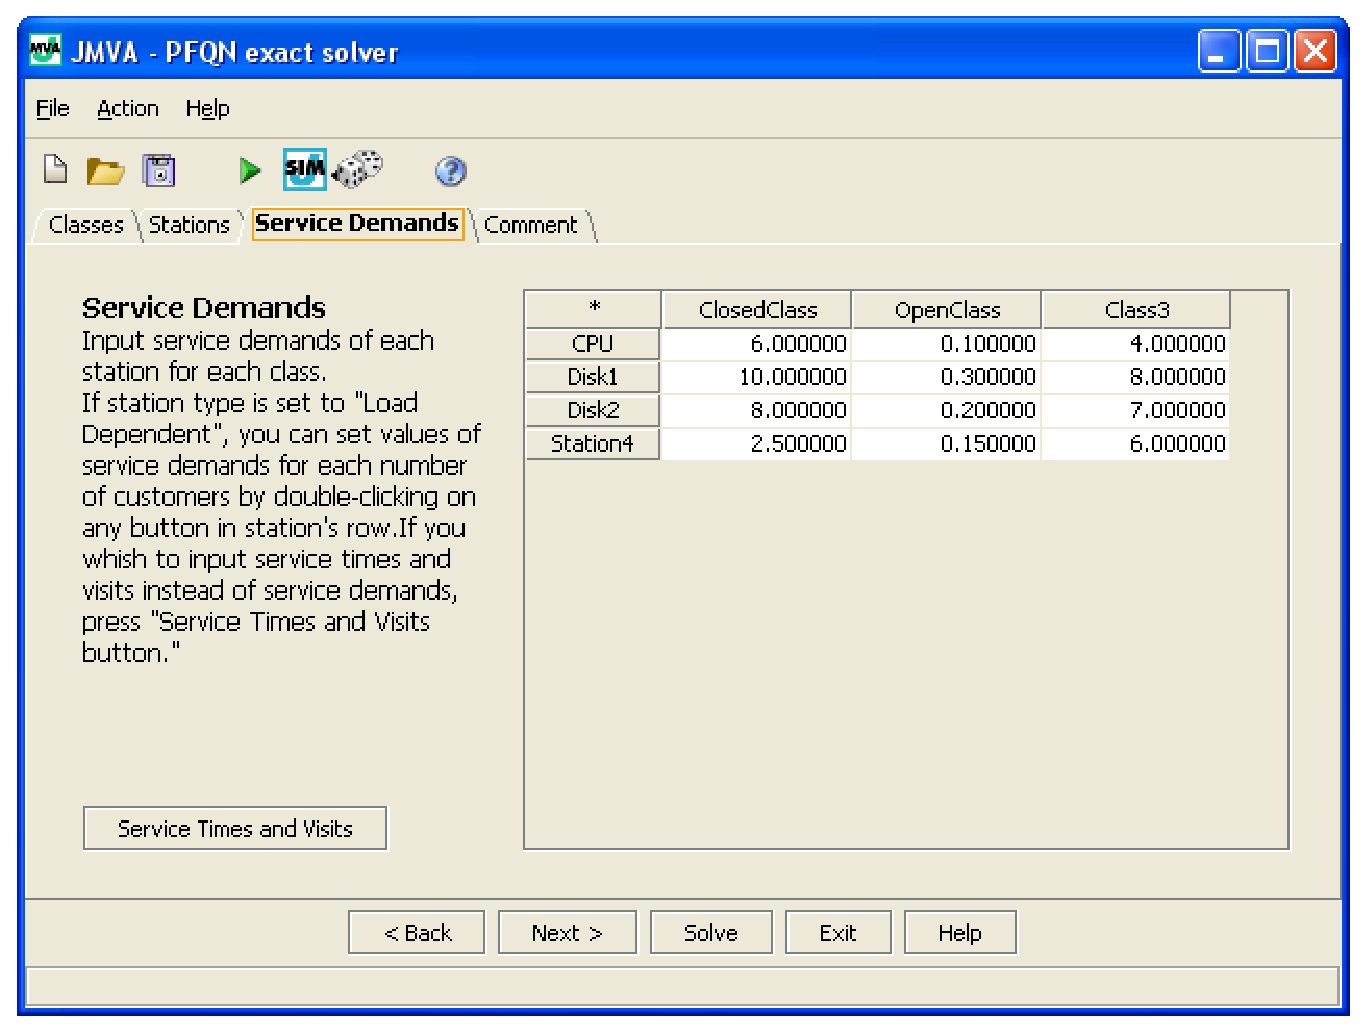
\includegraphics[scale=.5]{img/jmva/serviceDemands}
    \end{center}
    \caption{The Service Demands Tab}
    \label{fig:jmva:ServiceDemandsTab}
\end{figure}

In the example of \autoref{fig:jmva:ServiceDemandsTab}, each job of
type \emph{ClosedClass} requires an average service demand time of 6
sec to \emph{CPU}, 10 sec to \emph{Disk1}, 8 sec to
\emph{Disk2} and 2.5 sec to \emph{Station4}.\\
On the other hand, a job of type \emph{OpenClass} requires on
average 0.1 sec of \emph{CPU} time, 0.3 sec of \emph{Disk1} time,
0.2 sec of \emph{Disk2} time and 0.15 sec of \emph{Station4} time to
be processed by the system.

If the model contains any load dependent station, the behavior of
\autoref{fig:jmva:LD} will be shown.

\begin{figure}[htbp]
    \begin{center}
        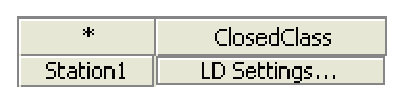
\includegraphics[scale=.5]{img/jmva/ld}
    \end{center}
    \caption{Defining a \emph{load dependent} station service demand}
    \label{fig:jmva:LD}
\end{figure}

By double-clicking on \emph{LD Settings\dots} button a window will
show up and that can be used to insert the values of the service
demands for each possible number of customer inside the station.
That values can be computed by evaluating an analytic function as
shown in \autoref{fig:jmva:LDEdit}. The list of supported operators
and more details are reported in \autoref{sec:jmva:JEP}.

\begin{figure}[htbp]
    \begin{center}
        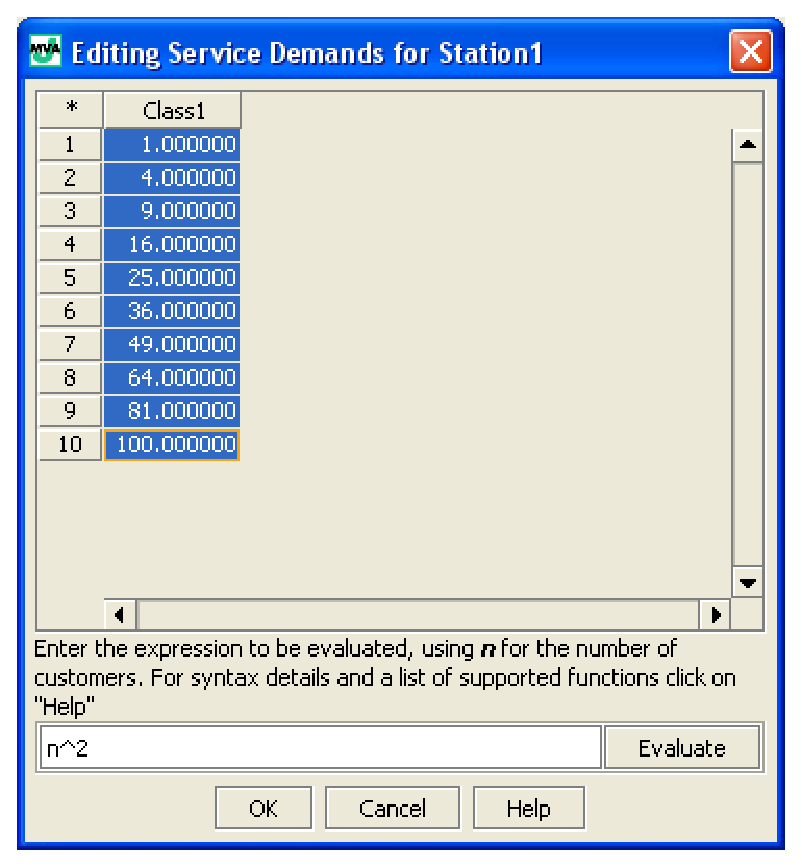
\includegraphics[scale=.5]{img/jmva/ldEdit}
    \end{center}
    \caption{Load Dependent editing window}
    \label{fig:jmva:LDEdit}
\end{figure}

\subsubsection{Service Times and Visits Tabs}
In the former tab you can insert the Service Times $S_{kc}$ for each
pair \{station~$k$-class~$c$\} in the model, in the latter you can
enter the visits number $V_{kc}$ (See \autoref{fig:jmva:visits}).

\begin{figure}[htbp]
    \begin{center}
        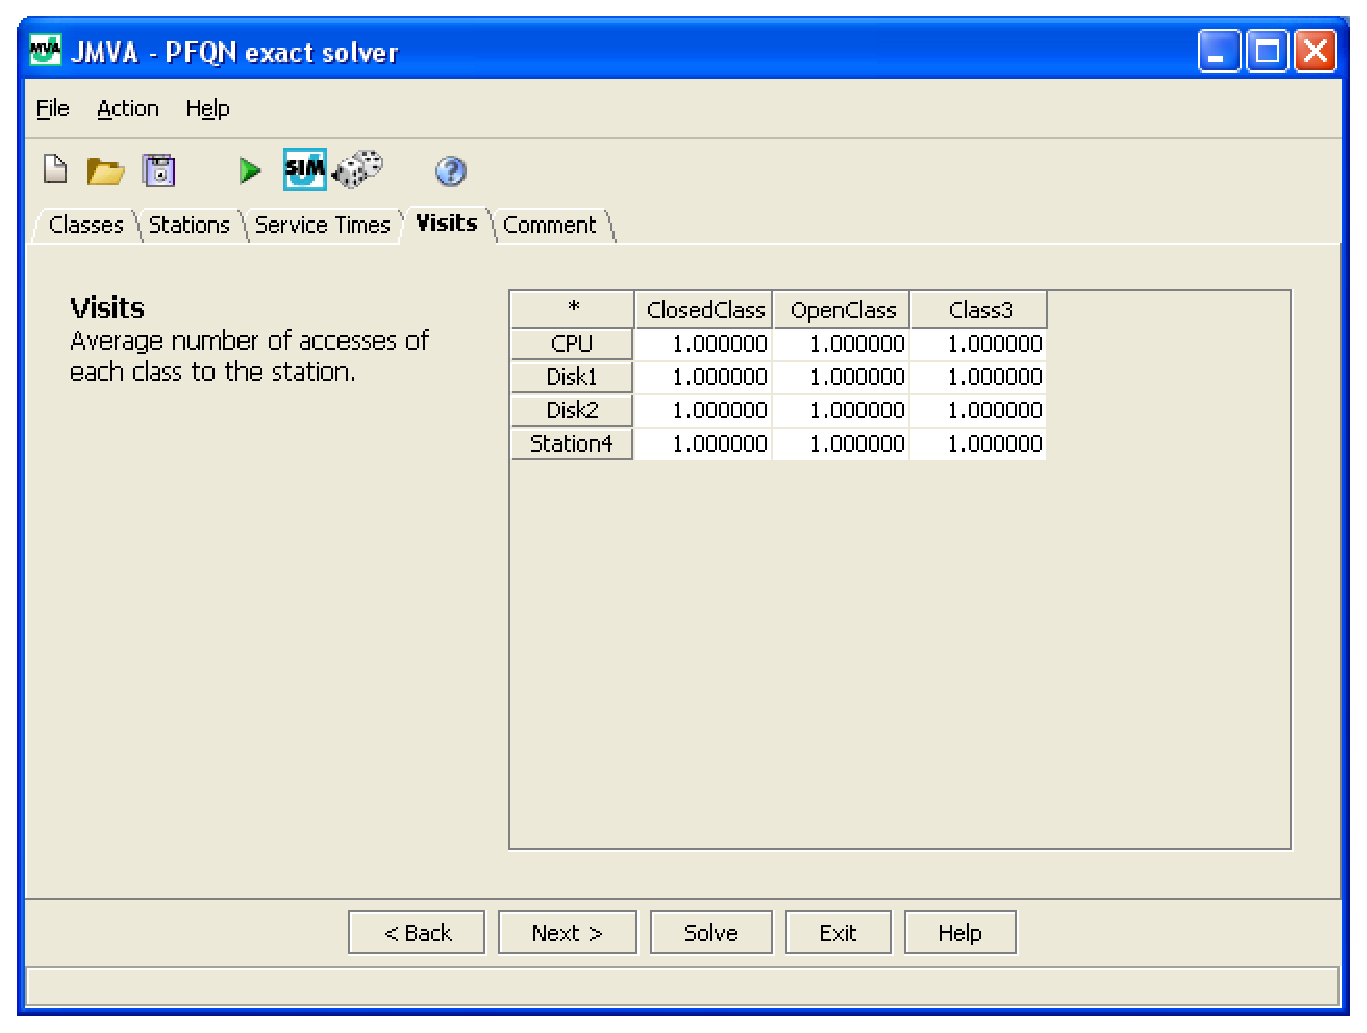
\includegraphics[scale=.5]{img/jmva/visits}
    \end{center}
    \caption{Visits Tab}
    \label{fig:jmva:visits}
\end{figure}

The layout of these tabs is similar to the one of the
\texttt{Service Demand Tab} described in the previous paragraph. The
default value for each element of the Service Times ($S$) matrix is
zero, while it's one for Visits' matrix elements.

In current model contains load dependent stations, the behavior of
\texttt{Service Times Tab} for their parametrization will be
identical to the one described on the previous paragraph for
\texttt{Service Demands Tab}. On the other hand \texttt{Visits Tab}
behavior won't change as load dependency is a property of service
times and not of visits.

\subsection{What-if Tab}
\label{sec:jmva:whatif} This Tab is used to perform a what-if
analysis, i.e. solve multiple models changing the value of a
\texttt{control parameter}. In \autoref{fig:jmva:whatifDisabled} is
shown this panel when what-if analysis is disabled.

\begin{figure}[htbp]
    \begin{center}
        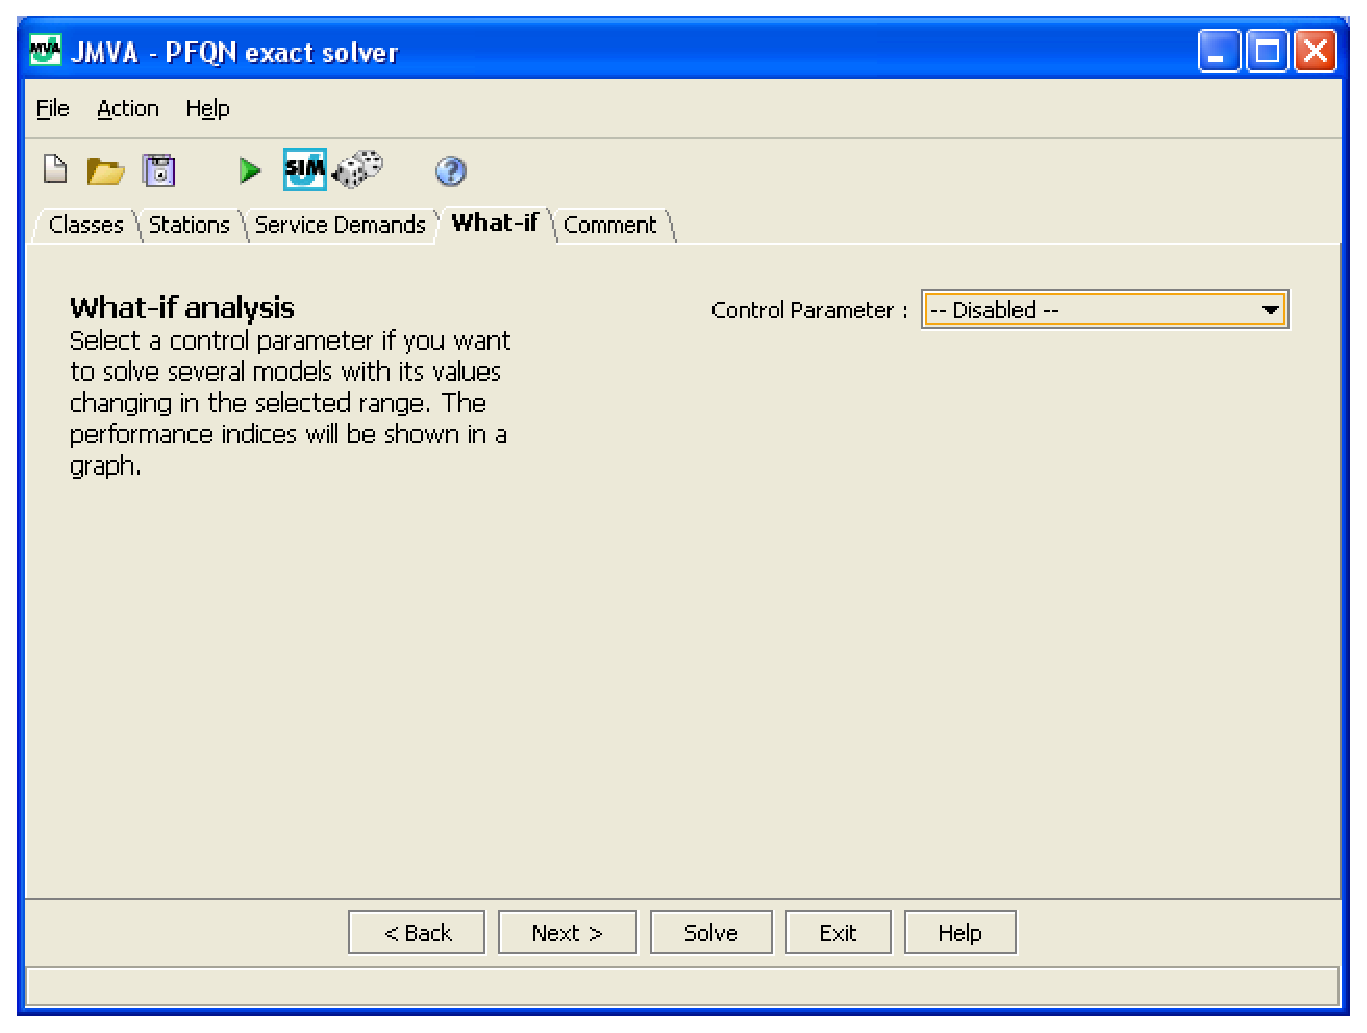
\includegraphics[scale=.5]{img/jmva/whatifDisabled}
    \end{center}
    \caption{What-if Tab - Disabled analysis}
    \label{fig:jmva:whatifDisabled}
\end{figure}

The first parameter to be set is the \texttt{control parameter} i.e.
the parameter that will be changed to solve different models in a
selected range. Five choices are possible:
\begin{description*}
\item[Disabled :] disables what-if analysis, so only a single queueing network
model, specified in the previous steps, will be solved. This is the
\emph{default} option.
\item[Customer Numbers :] different models will be
executed by changing the \texttt{number of customers} of a single
\texttt{closed} class or of every closed class proportionally. This
option is available only when current model has at least one closed
class.
\item[Arrival Rates :] different models will be
executed by changing \texttt{arrival rate} of a single \texttt{open}
class or of every open class proportionally. This option is
available only when current model has at least one open class.
\item[Population Mix :] the total number of customers will be kept
constant, but the population mix (i.e. the ratio between
\texttt{number of customers} of selected closed class $i$ and the
total number of customers in the system $\beta_i = N_i / \sum_k
N_k$). This option is available only when current model has two
closed classes.
\item[Service Demands :] different models will be solved changing
the \texttt{service demand} value of a given station for a given
class or for all classes proportionally. This option is available
only for \texttt{load independent} and \texttt{delay} stations.
\end{description*}

Whenever a control parameter is selected, the window layout will be
changed to allow the selection of a valid range of values for it.
For example in \autoref{fig:jmva:whatifDemands} \texttt{Service
Demands} control parameter was selected. On the bottom of the
window, a riepilogative table is presented: depending on selected
control parameter, that table is used to show the \emph{initial
state} of involved parameters. Every class currently selected for
what-if analysis is shown in red.

\begin{figure}[htbp]
    \begin{center}
        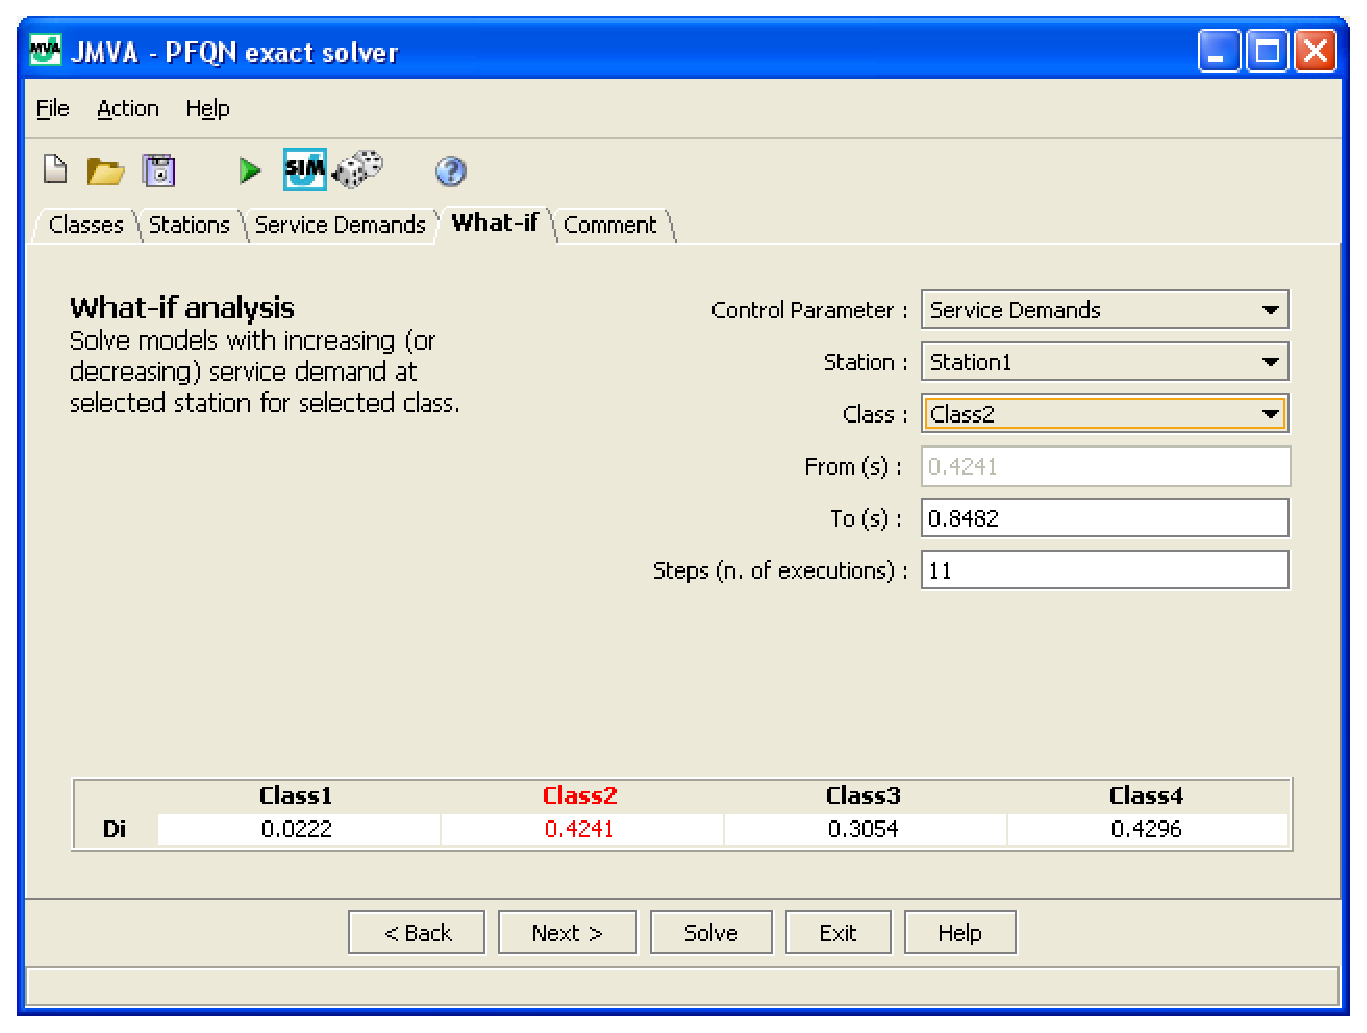
\includegraphics[scale=.5]{img/jmva/whatifDemands}
    \end{center}
    \caption{What-if Tab - Service Demands}
    \label{fig:jmva:whatifDemands}
\end{figure}

A brief description of each field is now presented:
\begin{description*}
\item[Station :] available only with \texttt{Service Demands} control
parameter. This combo box allows to select at which station service
demand values will be modified.
\item[Class :] allow to select for which class the selected
parameter will be changed. A special value, namely \texttt{All
classes proportionally}, is used to modify the control parameter for
each class keeping constant the proportion between different
classes\footnote{for example, in a model with two closed classes
with population vector (2,6), the following models can be executed:
(1,3), (2,6), (3,9), (4, 12), \dots}. This special value is not
available in \texttt{Population Mix} analysis as we are changing the
proportion of jobs between two closed classes.
\item[From :] the initial value of what-if analysis. It was chosen
to leave this value fixed to the initial value specified by the user
in the previous steps to avoid confusions, so this field acts as a
reminder. The only exception is when \texttt{Population Mix} is
changed, in that case it's allowed to modify this value too.
\item[To :] the final value of what-if analysis. Please notice that
this value can be greater or smaller than \texttt{From} value and is
expressed in the same measure unit. Whenever \texttt{All classes
proportionally} option is selected, both \texttt{From} and
\texttt{To} values are expressed as percentages of initial values
(specified in the previous steps and reminded in the table at the
bottom of the panel, see \autoref{fig:jmva:whatifDemands}), in the
other situations they are considered as absolute values for the
chosen parameter.
\item[Steps :] this is chosen number of executions i.e. the number
of different models that will be solved. When control parameter is
\texttt{Customer Numbers} or \texttt{Population Mix}, the model can
be correctly specified only for integer values of population. JMVA
will perform a fast computation to find the maximum allowed number
of executions given current \texttt{From} and \texttt{To} values: if
user specify a value bigger than that, JMVA will use the computed
value.
\end{description*}


\subsection{Comment Tab}
In this Tab, a short - optional - comment about the model can be
inserted; it will be saved with the other model parameters.

\subsection{Expression Evaluator}
\label{sec:jmva:JEP} An expression evaluator is used for the
definition of service demands or service times of a load dependent
station. It allows to specify times as an analytic function of $n$
where $n$ is the number of customer inside the station.

Expression are evaluated using
\emph{JEPLite}\footnote{http://jeplite.sourceforge.net/} (Java Math
Expression Parser enlited) package which supports all operators
enumerated in \autoref{tab:jmva:Operators} and all functions
enumerated in \autoref{tab:jmva:Functions}.

\begin{table}[htbp]
\begin{center}
\begin{tabular}{|c|c|}
Operator & Symbol\\
\hline
Power & $^{\wedge}$\\
Unary Plus, Unary Minus & $+n$, $-n$\\
Modulus & $\%$\\
Division & $/$ \\
Multiplication & $*$\\
Addition, Subtraction & $+$, $-$\\
\hline
\end{tabular}
\end{center}
\caption{List of all supported operators ordered by priority}
\label{tab:jmva:Operators}
\end{table}

\begin{table}[htbp]
\begin{center}
\begin{tabular}{|c|c|}
Function & Symbol\\
\hline
Sine & sin()\\
Cosine & cos()\\
Tangent & tan()\\
Arc Sine & asin()\\
Arc Cosine & acos()\\
Arc Tangent & atan()\\
Hyperbolic Sine & sinh()\\
Hyperbolic Cosine & cosh()\\
Hyperbolic Tangent & tanh()\\
Inverse Hyperbolic Sine & asinh()\\
Inverse Hyperbolic Cosine & acosh()\\
Inverse Hyperbolic Tangent & atanh()\\
Natural Logarithm & ln()\\
Logarithm base 10 & log()\\
Absolute Value / Magnitude & abs()\\
Random number $[0,1]$ & rand()\\
Square Root & sqrt()\\
Sum & sum()\\
\hline
\end{tabular}
\end{center}
\caption{List of supported functions for the load dependent service
times} \label{tab:jmva:Functions}
\end{table}

\subsection{Model Solution}
\label{sec:jmva:solution}Use \texttt{Solve} command to solve the
model. If the model specify a what-if analysis, please refer to
\autoref{sec:jmva:solutionWhatif}. Model results will be shown on a
separate window, like the one of \autoref{fig:jmva:results}.

\begin{figure}[htbp]
    \begin{center}
        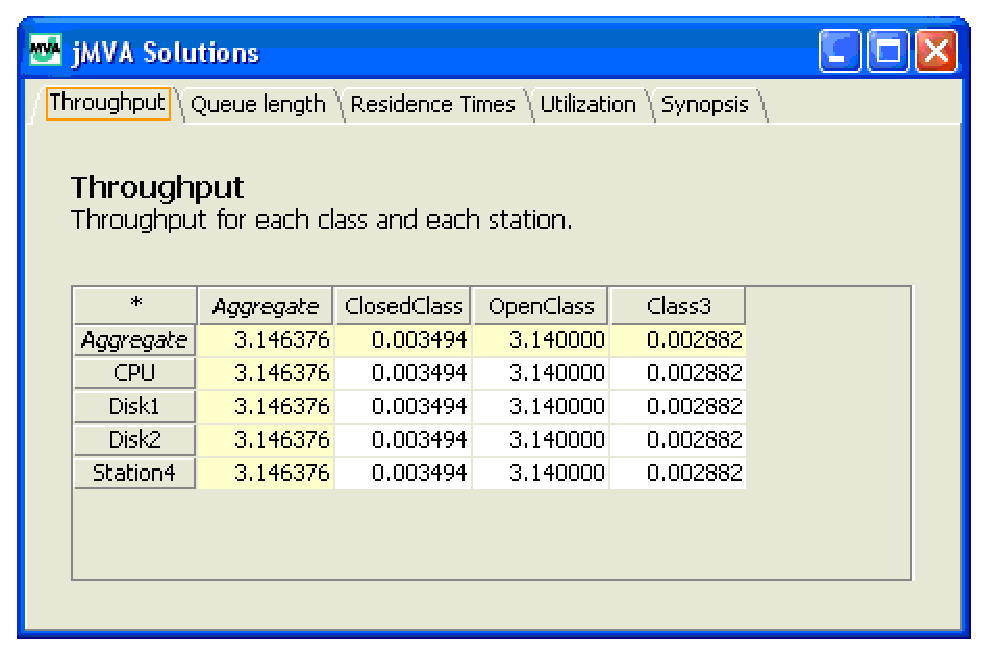
\includegraphics[scale=.5]{img/jmva/results}
    \end{center}
    \caption{Model Solution (Throughput Tab)}
    \label{fig:jmva:results}
\end{figure}

Using the tab selector, all the other computed performance indices
can be seen: Throughput, Queue lengths, Residence Times,
Utilizations and a synopsis panel with schematic report of input
model. Both results and synopsis tab data can be copied to clipboard
with \texttt{CTRL+C} keyboard shortcut.

When open classes are used, the resource saturation control is
performed. For multiple class models, the following inequality must
be satisfied:
\[
{\max_k {\sum_c{\lambda_c * D_{kc}}}} < 1
\]
This inequality ensures that no service center is saturated as a
result of the combined loads of all the classes. Let us consider, as
example, the model with the classes shown in
\autoref{fig:jmva:3Classes} with the D-matrix shown in
\autoref{fig:jmva:ServiceDemandsTab} Since $\lambda = 3.14 < 3.33 =
1 / 0.3 = 1 / D_{max}$ the model is not in saturation and the
\texttt{Solve} command will be executed correctly.

In this example, substituting $D_{\textrm{Disk1-OpenClass}}$ with
values $\geq 1/3.14 \approx 0.318$ will cause the saturation of
resource \emph{Disk1} and the error message of
\autoref{fig:jmva:saturation} will appear.

\begin{figure}[htbp]
    \begin{center}
        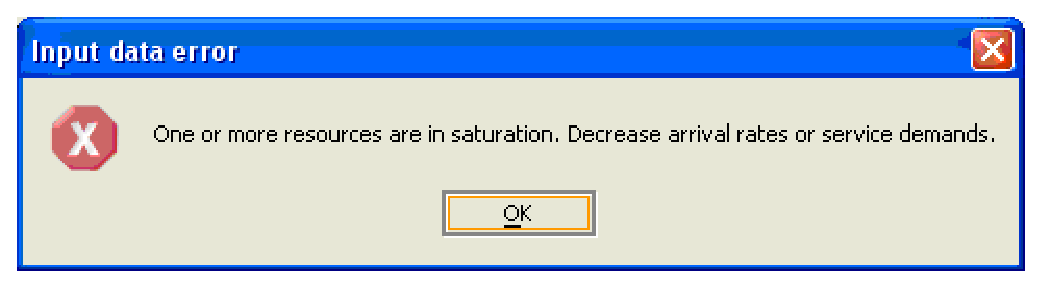
\includegraphics[scale=.5]{img/jmva/saturation}
    \end{center}
    \caption{Input data error message }
    \label{fig:jmva:saturation}
\end{figure}

\subsection{Model Solution - What-if analysis}
\label{sec:jmva:solutionWhatif}Use \texttt{Solve} command to solve
the model. During model solution, a progress window, see
\autoref{fig:jmva:progress}, shows up. It displays the cumulative
number of models currently solved, the total number of models to be
solved and the elapsed time.

\begin{figure}[htbp]
    \begin{center}
        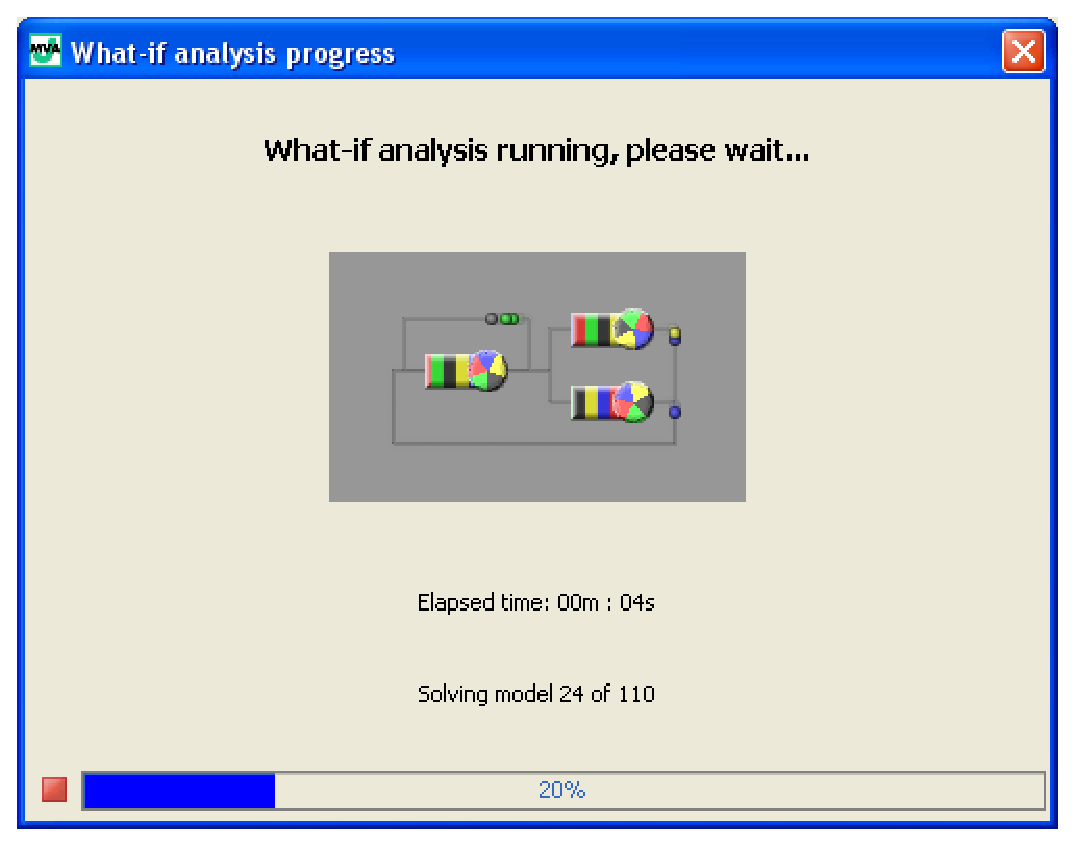
\includegraphics[scale=.5]{img/jmva/progress}
    \end{center}
    \caption{Model Solution progress window}
    \label{fig:jmva:progress}
\end{figure}

At the end of the solution, results will be shown in a separate
window, see \autoref{fig:jmva:graphical}.
\begin{figure}[htbp]
    \begin{center}
        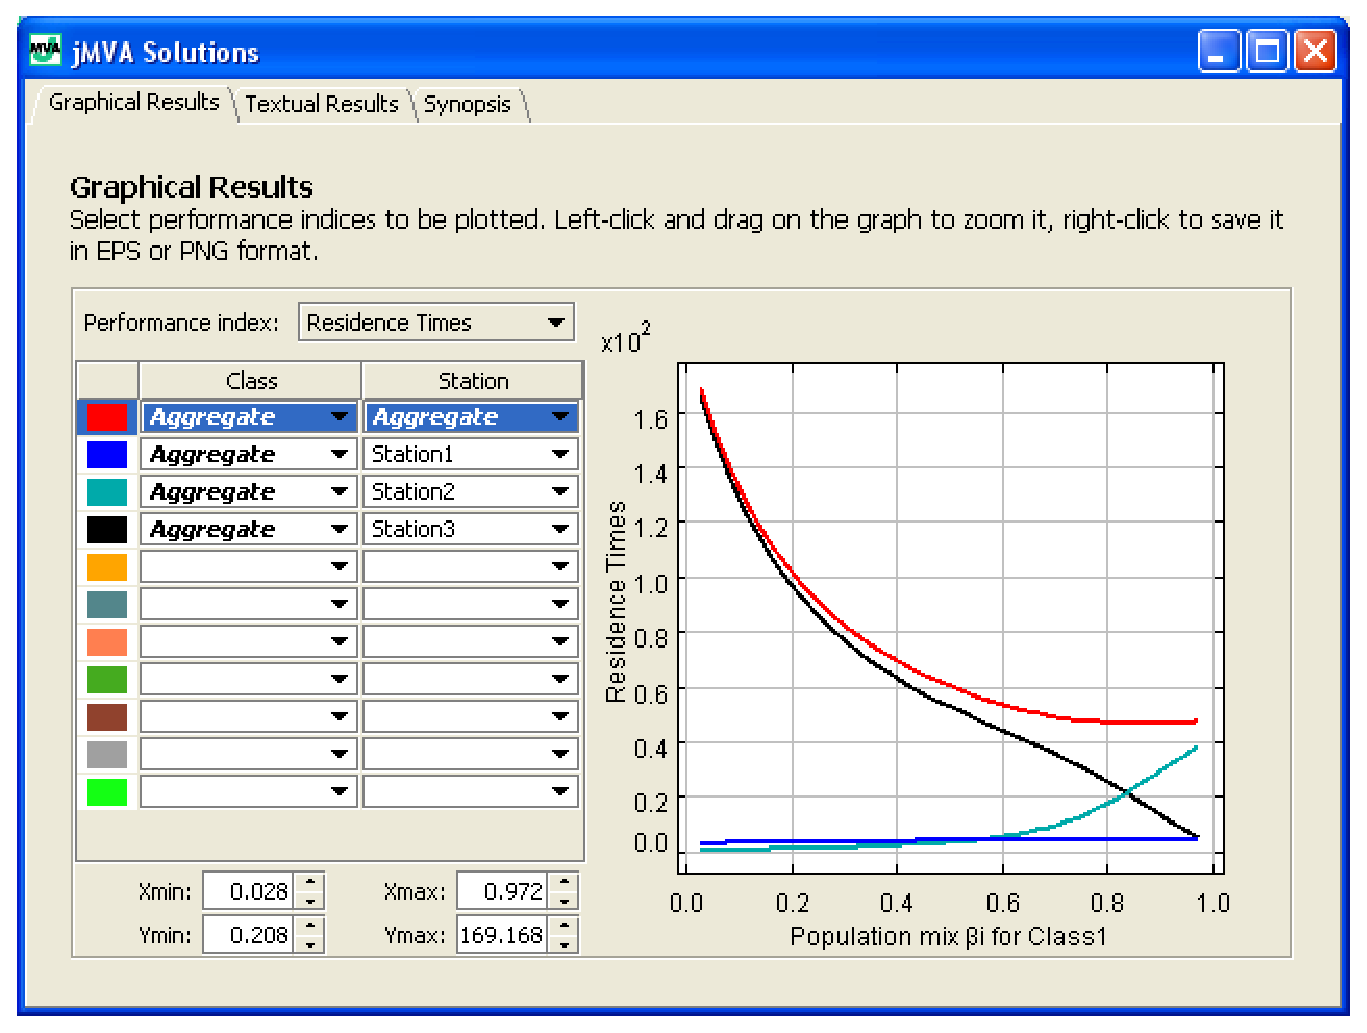
\includegraphics[scale=.5]{img/jmva/Graphical}
    \end{center}
    \caption{Model Solution - Graphical Results Tab}
    \label{fig:jmva:graphical}
\end{figure}
This tab allows to show in a plot the relation between the chosen
control parameter (see \autoref{sec:jmva:whatif}) and the
performance indices computed by the analytic engine.

The combo box \texttt{Performance Index} allows to select the
performance index to be plotted in the graph, while in the table
below, users can select the resource and the class considered.
\begin{itemize*}
\item The first column is fixed and lists all available colors to be
used in the graph.
\item The second column, named \texttt{Class}, is used to select the
class considered in the graph. The special value \texttt{Aggregate}
is used for the aggregate measure for all classes. If input model is
single-class, the class is selected by default for each row.
\item The final column, named \texttt{Station}, is used to select the
station considered in the graph. The special value
\texttt{Aggregate} is used for the aggregate measure for the entire
network. Note that the \texttt{Aggregate} value is not valid when
the \texttt{Utilization} performance index is selected.
\end{itemize*}

In addition to the \emph{center} performance indices (i.e.
\texttt{Throughput}, \texttt{Queue length}, \texttt{Residence
Times}, \texttt{Utilization}), three \emph{system} performance
indices are provided  in the \texttt{Performance Index} combo box
(\texttt{System Response Time}, \texttt{System Throughput},
\texttt{Number of Customers}). This \emph{system} indices can be
easily obtained by selecting the special \texttt{Aggregate} value
for both \texttt{Class} and \texttt{Station} columns of the
corresponding center indices (see \autoref{cha:glossary} for the
definition of the performance indices), but they were provided here
as a \emph{shortcut}. As we are referring to aggregate measures, the
selection of reference class and station is not significant and, in
this case, the table in the left of \autoref{fig:jmva:graphical}
will not be shown.

On the bottom-left corner of the window, users can modify minimum
and maximum value of both X and Y axis of the plot. JMVA is designed
to automatically best-fit the plot in the window but this controls
allow the user to specify a custom range or zoom on the plot.
Another fast method to perform a zoom operation is to left-click and
drag a rectangle on the graphic window (see
\autoref{fig:jmva:zoomDrag}) or right-click on it and select
\texttt{Zoom in} or \texttt{Zoom out} options. To automatically
reset the best-fit scale users can right-click on the graphic window
and select \texttt{Original view} option.

\begin{figure}[htbp]
    \begin{center}
        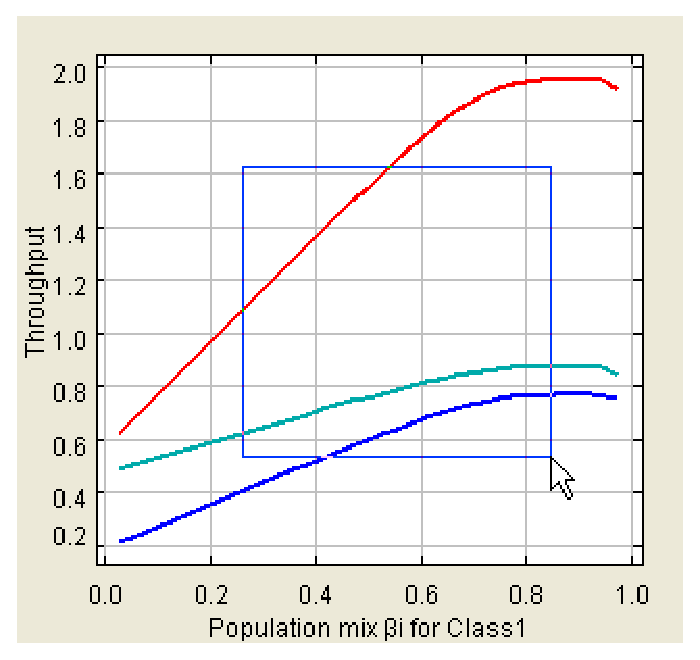
\includegraphics[scale=.5]{img/jmva/whatIfDrag}
    \end{center}
    \caption{Zoom operation on the plot}
    \label{fig:jmva:zoomDrag}
\end{figure}

The graphic window allows to export plots as image to be included in
documents and presentations. To save current graph as image,
right-click on the graphic and select \texttt{Save as\dots} option.
A dialog will be shown to request the name of the file and the
format. Currently supported format are Portable Network Graphics -
PNG - (raster) and Encapsulated PostScript - EPS - (vectorial,
currently only black and white).

The second tab of the solution window, shown in
\autoref{fig:jmva:textualResults}, is used to display the solutions
of each execution of the analytic algorithm.

\begin{figure}[htbp]
    \begin{center}
        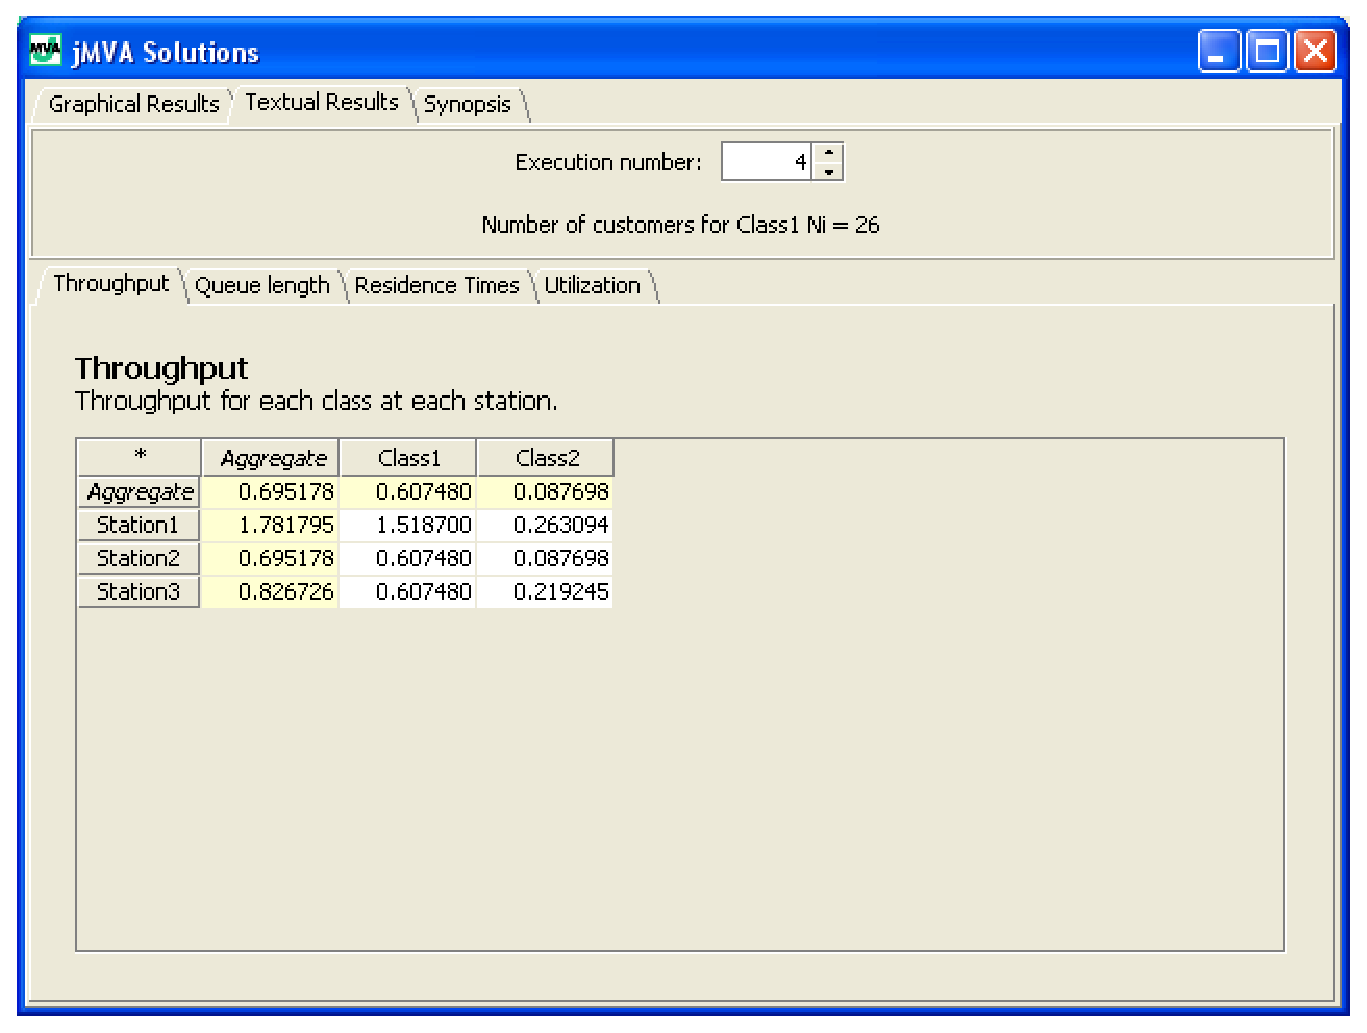
\includegraphics[scale=.5]{img/jmva/textualResults}
    \end{center}
    \caption{Model Solution - Textual Results Tab}
    \label{fig:jmva:textualResults}
\end{figure}

This Tab has the same structure of the results window without
What-if analysis (described in \autoref{sec:jmva:solution}) but
allows to select the execution to be shown in the field
\texttt{Execution Number}. By entering requested execution number in
the spinner, or using the \emph{up} and \emph{down} arrows, user can
cycle between all the computed performance indices for each
execution. Just below the spinner, a label gives information on the
value of the control parameter for the currently selected execution.

\subsection{Modification of a model}
To modify system parameters return to the main window and enter new
data. After the modifications, if you use \texttt{Solve} command, a
new window with model result will show. You can \texttt{save} this
new model with the previous name - overwriting the previous one - or
\texttt{save} it with a different name or in a different directory.

\section{Menu entries}
\label{sec:jmva:Menu}
\subsection{File}
\subsubsection{New}
Use this command in order to create a new JMVA model.

\noindent
\begin{tabular}{ll}
Shortcut on Toolbar: & 
\includegraphics[scale=.8]{img/jmva/new}\\
Accelerator Key: & CTRL+N
\end{tabular}

\subsubsection{Open}
Use this command to open an existing model. You can only open one
model at time, to edit two or more models start more than one
instance of JMVA. If current model was modified since its creation
or last save action, a popup window will be shown for confirmation.

It's possible to open not only models saved with JMVA (*.jmva), but
also with other programs of the suite (for example JABA *.jaba, JSIM
*.jsim and JMODEL *.jmodel). Whenever a foreign data file is opened, a
conversion is performed and error/warnings occurred during
conversion will be reported in a window.

Models are stored in XML format, see \emph{JMT system manual} for a
detailed description.

\noindent
\begin{tabular}{ll}
Shortcut on Toolbar: & 
\includegraphics[scale=.8]{img/jmva/open}\\
Accelerator Key: & CTRL+O
\end{tabular}

\subsubsection{Save}
Use this command in order to save the active document with its
current name in the selected directory.

When you save a document for the first time, JMVA displays the Save
As dialog box so you can rename your document. If you save a model
after its resolution, results are stored with model definition data.

\noindent
\begin{tabular}{ll}
Shortcut on Toolbar: & 
\includegraphics[scale=.8]{img/jmva/save}\\
Accelerator Key: & CTRL+S
\end{tabular}

\subsubsection{Exit}
Use this command in order to end a JMVA session. You can also use
the Close command on the application Control menu. If current model
was modified since its creation or last save action, a popup window
will be shown for confirmation.

\noindent
\begin{tabular}{ll}
\\
Accelerator Key: & CTRL+Q
\end{tabular}

\subsection{Action}
\subsubsection{Solve}
Use this command when model description is terminated and you want
to start the solution of the model. At the end of the process the
window in \autoref{fig:jmva:results} will popup.

\noindent
\begin{tabular}{ll}
Shortcut on Toolbar: & 
\includegraphics[scale=.8]{img/jmva/solve}\\
Accelerator Key: & CTRL+L
\end{tabular}

\subsubsection{Randomize}
Use this command in order to insert random values into Service
Demands - or Service Times - table. Generated values are
automatically adjusted to avoid saturation of resources.

\noindent
\begin{tabular}{ll}
Shortcut on Toolbar: & 
\includegraphics[scale=.8]{img/jmva/randomize}\\
Accelerator Key: & CTRL+R
\end{tabular}

\subsubsection{Import in JSIM}
This command will import current model into JSIM to solve it using
simulator. A simple parallel topology is derived from number of
visits at each station and generated model is equivalent to original
one.

\noindent
\begin{tabular}{ll}
Shortcut on Toolbar: & 
\includegraphics[scale=.8]{img/jmva/toJSIM}\\
Accelerator Key: & CTRL+G
\end{tabular}

\subsection{Help}
\subsubsection{JMVA Help}
Use this command to display application help. From the initial
window, you can jump to step-by-step instructions that show how use
JMVA and consult various types of reference information.

Once you open Help, you can click the Content button whenever you
want to return to initial help window.

\noindent
\begin{tabular}{ll}
Shortcut on Toolbar: & 
\includegraphics[scale=.8]{img/jmva/help}\\
Accelerator Key: & CTRL+Q
\end{tabular}

\subsubsection{About}
Use it in order to display information about JMVA version and
credits.

\section{Examples}
In this section we will describe some examples of model
parametrization and solution using MVA exact solver. Step-by-step
instructions are provided in five examples:
\begin{enumerate*}
\item A single class closed model with three load independent stations and a delay service
center (\autoref{sec:jmva:example1})
\item A multiclass open model with two classes and three load independent
stations (\autoref{sec:jmva:example2})
\item A single class closed model with a load dependent station and
a delay (\autoref{sec:jmva:example3})
\item A multiclass mixed model with three stations (\autoref{sec:jmva:example4})
\item A multiclass closed model where a what-if analysis is used to find optimal
Population Mix values (\autoref{sec:jmva:example5})
\end{enumerate*}


\subsection{Example 1 - A model with a single closed class}
\label{sec:jmva:example1} Solve the single class model specified in
\autoref{fig:jmva:Example1topology}.
\begin{figure}[htbp]
    \begin{center}
        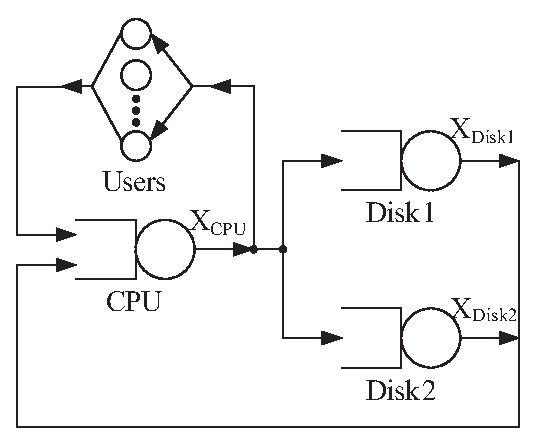
\includegraphics[scale=.65]{img/jmva/example1}
    \end{center}
    \caption{Example 1 - network topology}
    \label{fig:jmva:Example1topology}
\end{figure}
The customer class, named \emph{ClosedClass} has a population of $N
= 3$ customers.

There are four stations, three are of load independent type (named
\emph{CPU}, \emph{Disk1} and \emph{Disk2}) and one is of delay type
(named \emph{Users}). \emph{Users} delay station represents user's
\emph{think time} ($Z = 16$ s) between interaction with the system.
Service times and visits for stations are reported in
\autoref{tab:jmva:example1ServTimes}.

\begin{table}[htbp]
\begin{center}
\begin{tabular}{c|r|r|r|r|}
& \multicolumn{1}{c|}{CPU} & \multicolumn{1}{c|}{Disk1} & \multicolumn{1}{c|}{Disk2} & \multicolumn{1}{c|}{Users}\\
\hline
Service Times [s] & $0.006$ & $0.038$ & $0.030$ & $16.000$\\
Visits & $101.000$ & $60.000$ & $40.000$ & $1.000$\\
\hline
\end{tabular}
\end{center}
\caption{Example 1 - service times and visits}
\label{tab:jmva:example1ServTimes}
\end{table}

\subsubsection{Step 1 - Classes Tab}
\begin{itemize*}
\item use New command to create a new jMVA document
\item by default, you have already a \texttt{Closed} class
\item if you like, substitute default \emph{Class1} name with a customized
one (\emph{ClosedClass} in our example)
\item complete the table with workload intensity (number of customers). Remember that
intensity of a closed class N must be a positive integer number; in
this case, 3
\end{itemize*}

At the end of this step, the \texttt{Classes Tab} should look like
\autoref{fig:jmva:example1Classes}.

\begin{figure}[htbp]
    \begin{center}
        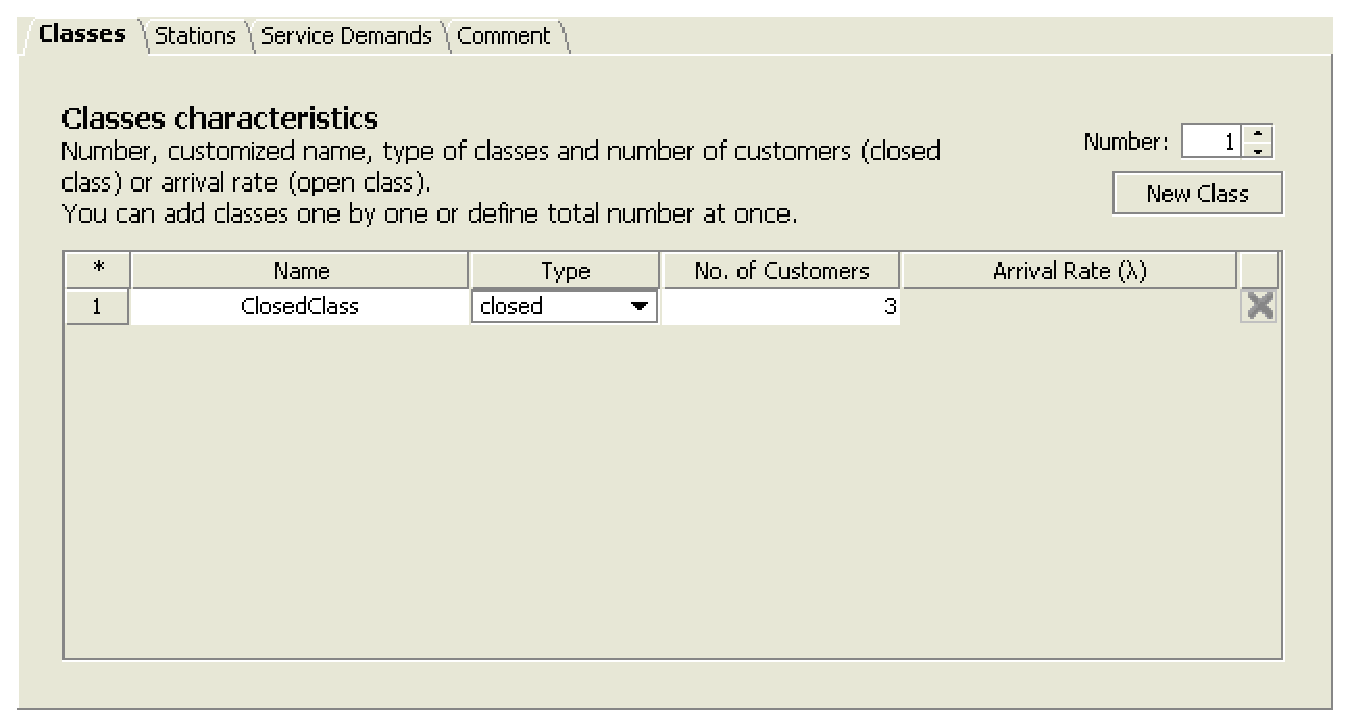
\includegraphics[scale=.5]{img/jmva/example1Class}
    \end{center}
    \caption{Example 1 - input data (Classes Tab)}
    \label{fig:jmva:example1Classes}
\end{figure}

\subsubsection{Step 2 - Stations Tab}
\begin{itemize*}
\item use \texttt{Next $>$} command to switch to \texttt{Stations Tab}
\item digit number 4 into stations number textbox or select number
4 using spin controls or push \emph{New Station} button three times.
Now your model has four \texttt{Load Independent} stations with a
default name
\item if you want you can change station names. Substitute \emph{CPU} for
default name \emph{Station1}, substitute \emph{Disk1} for default
name \emph{Station2}, substitute \emph{Disk2} for default name
\emph{Station3} and substitute \emph{Users} for default name
\emph{Station4}
\item change the type of last inserted station; \emph{Users} station is a
\texttt{Delay (Infinite Server)}
\end{itemize*}

At the end of this step, the \texttt{Stations Tab} should look like
\autoref{fig:jmva:example1Stations}.

\begin{figure}[htbp]
    \begin{center}
        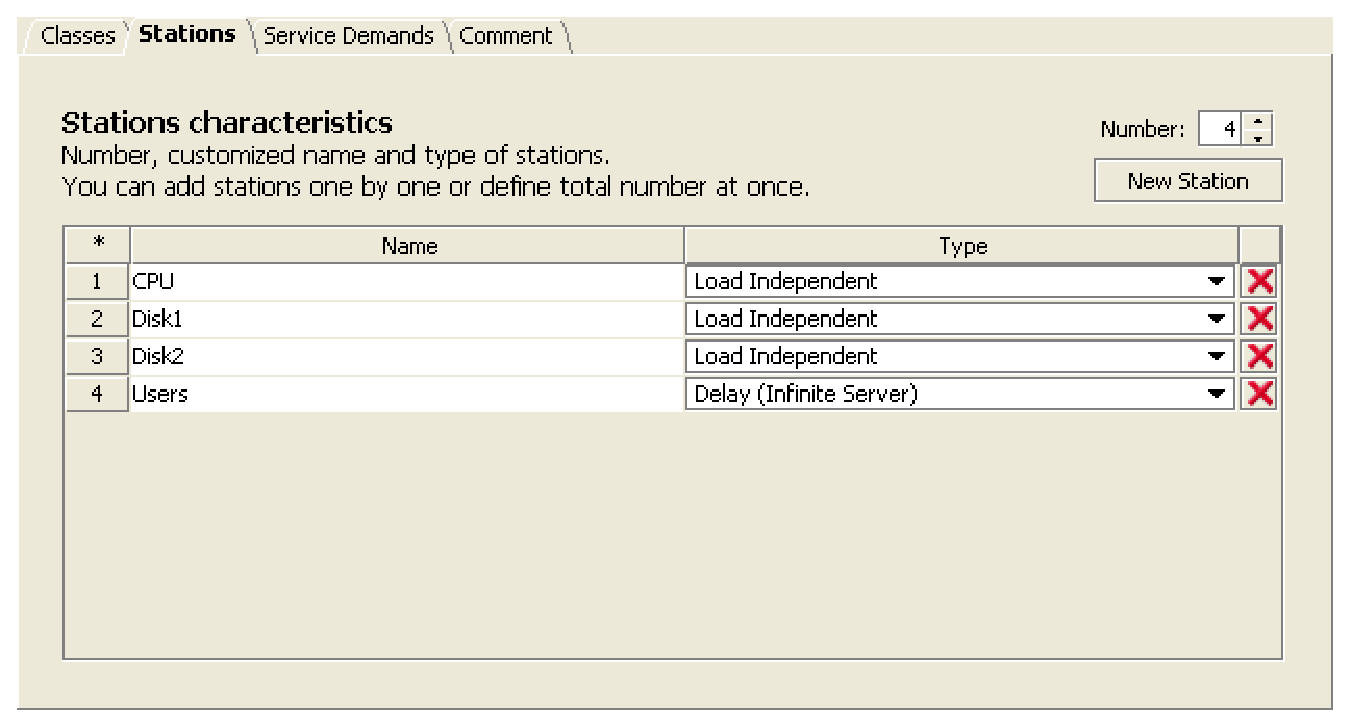
\includegraphics[scale=.5]{img/jmva/example1Stations}
    \end{center}
    \caption{Example 1 - input data (Stations Tab)}
    \label{fig:jmva:example1Stations}
\end{figure}

\subsubsection{Step 3 - Service Times and Visits Tabs}
\begin{itemize*}
\item use \texttt{Next $>$} command to switch to \texttt{Service Demands Tab}
\item press \emph{Service Time and Visit} button as you don't know
the Service Demands of the three stations: in this case Service
Times and number of Visits should be typed. After button pressure,
the \texttt{Service Demands Tab} will be hidden and \texttt{Service
times Tab} and \texttt{Visit Tab} will appear
\item you can input all Service Times in the table.
Remember that Service Time of the \emph{Users} station, of delay
type, is \emph{think time} $Z$, in this case $16$ s
\end{itemize*}

At this point, the \texttt{Service Times Tab} should look like
\autoref{fig:jmva:example1Service}.

\begin{figure}[htbp]
    \begin{center}
        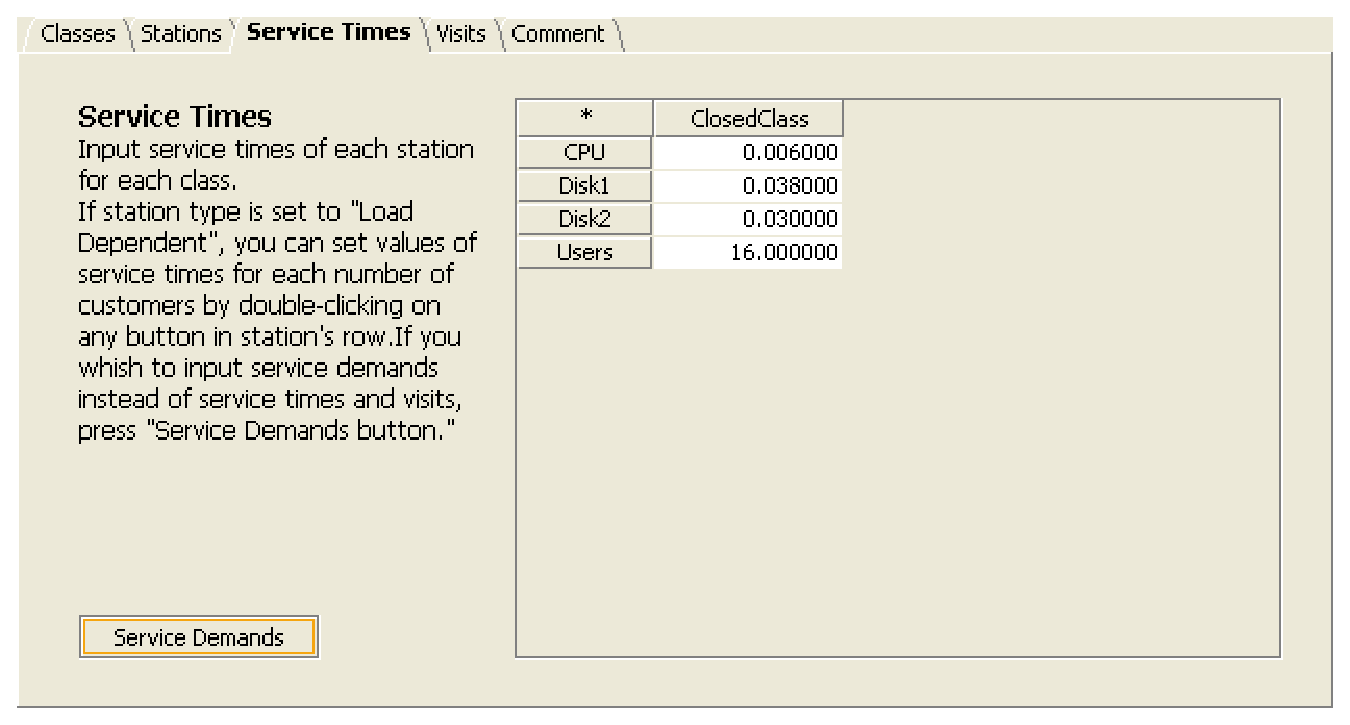
\includegraphics[scale=.5]{img/jmva/example1Service}
    \end{center}
    \caption{Example 1 - input data (Service Times Tab)}
    \label{fig:jmva:example1Service}
\end{figure}

\begin{itemize*}
\item use \texttt{Next $>$} command to switch to \texttt{Visits Tab}
\item input numbers of visits for all centers in the
table. In this case the number of visits of the \emph{Users}, the
infinite server station, is equal to 1 since a customer at the end
of an interaction with the system visits this station.
\end{itemize*}

At the end of this step, the \texttt{Visits Tab} looks like
\autoref{fig:jmva:example1Visits}.

\begin{figure}[htbp]
    \begin{center}
        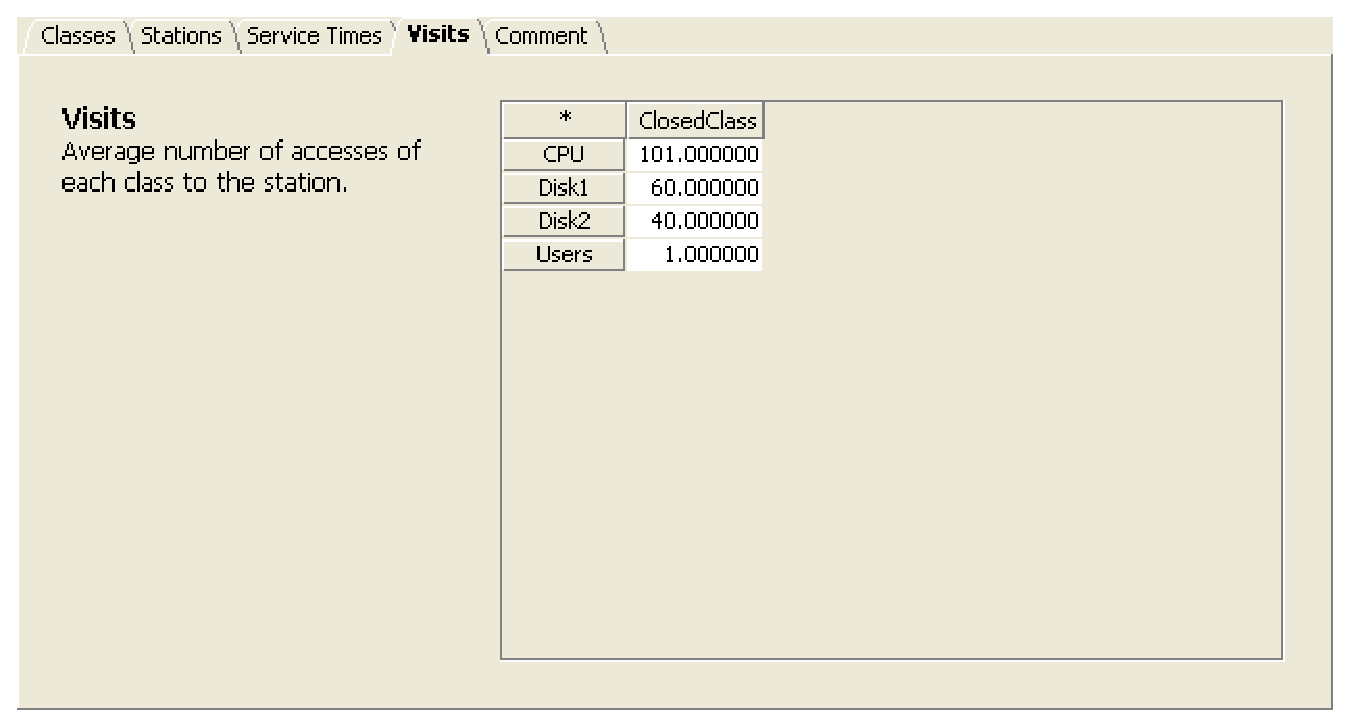
\includegraphics[scale=.5]{img/jmva/example1Visits}
    \end{center}
    \caption{Example 1 - input data (Visits Tab)}
    \label{fig:jmva:example1Visits}
\end{figure}

\subsubsection{Step 4 - Model Resolution}

Use \texttt{Solve} command to start the solution of the input model.
Model results will be displayed in a new window like the one of
\autoref{fig:jmva:example1Throughput}.

\begin{figure}[htbp]
    \begin{center}
        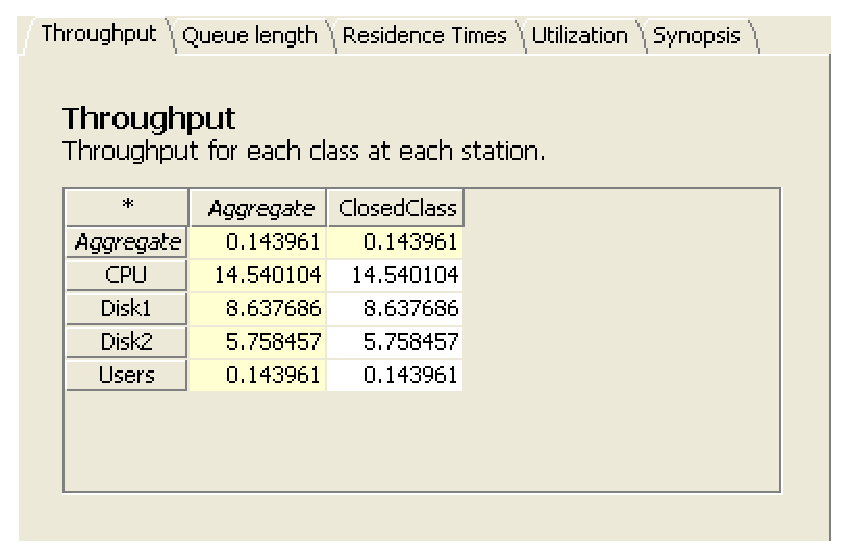
\includegraphics[scale=.5]{img/jmva/example1throughput}
    \end{center}
    \caption{Example 1 - output data (Throughput Tab)}
    \label{fig:jmva:example1Throughput}
\end{figure}

Since we are considering a single-class model, all results in the
column \emph{Aggregate} correspond to the results in the
\emph{ClosedClass} column.

JMVA computes Residence Times $W_k$, Throughputs $X_k$, Queue
lengths $Q_k$ and Utilizations $U_k$ for all stations. The algorithm
begins with the known solution for the network with zero customers,
and iterates on $N$ that, in this example, is three. Note that the
aggregate \emph{Residence Time} is the \emph{System Response Time}
measure and the aggregate \emph{Queue Length} is the average number
of customers in the system.

Using tab selector, you can change tab and see Queue length,
Residence Times, Utilizations and a synopsis panel with a schematic
report of the model (\autoref{fig:jmva:example1results}).

\begin{figure}[htbp]
    \begin{center}
        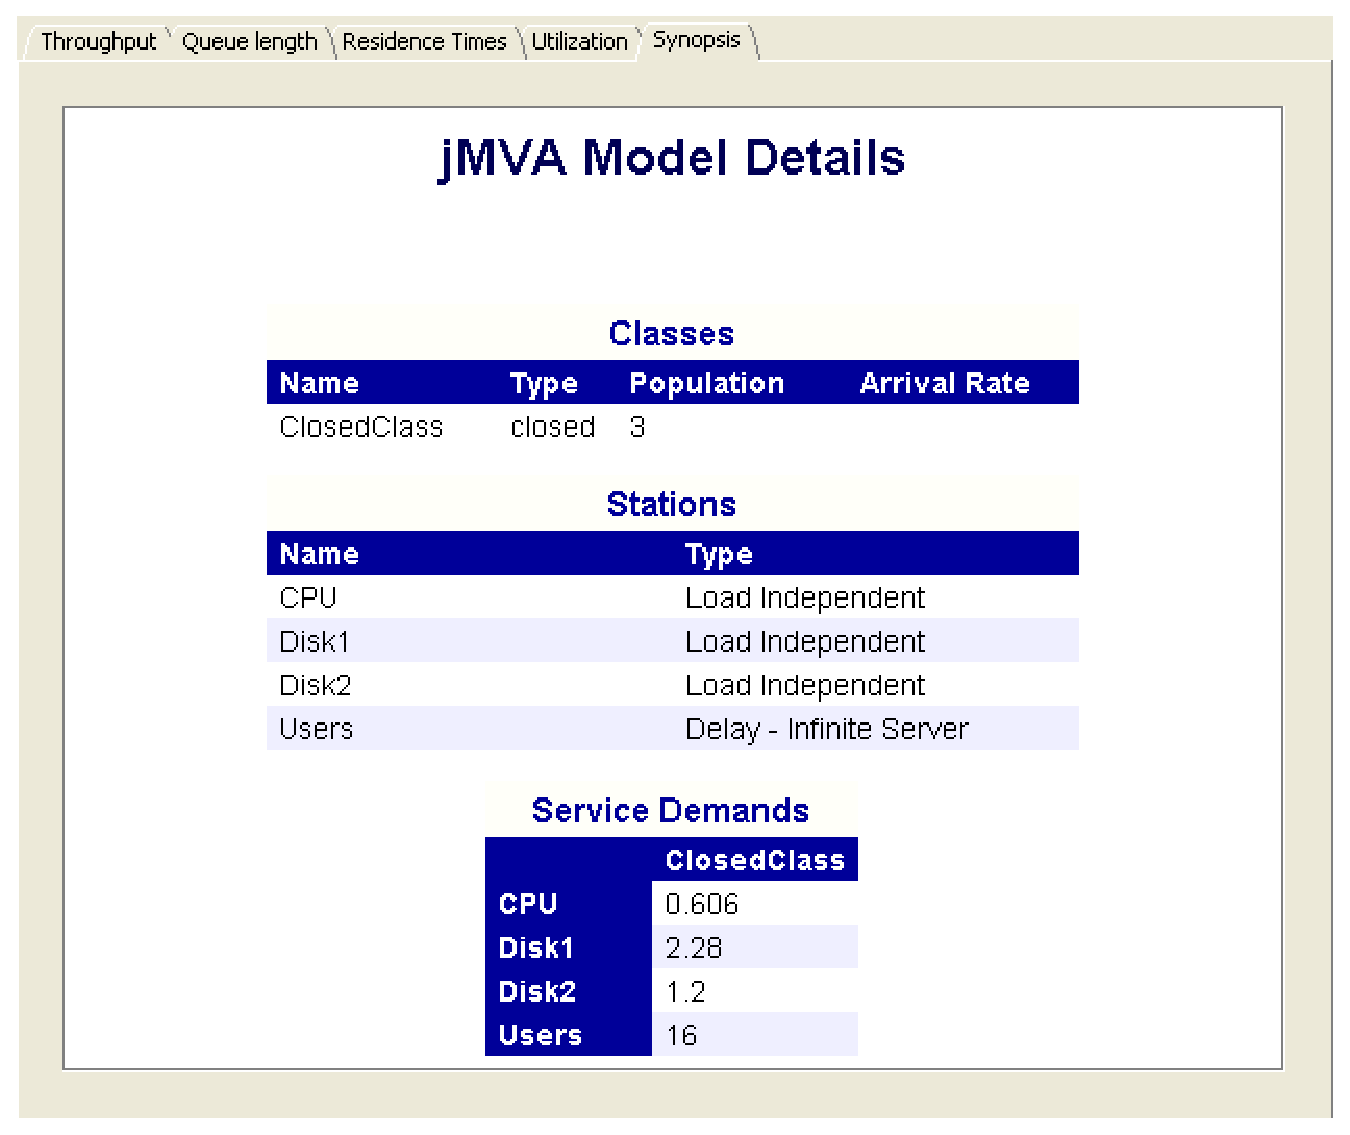
\includegraphics[scale=.5]{img/jmva/example1results}
    \end{center}
    \caption{Example 1 - output data (Synopsis Tab)}
    \label{fig:jmva:example1results}
\end{figure}

The computed performance indices are shown in
\autoref{tab:jmva:example1results}.

\begin{table}[htbp]
\begin{center}
\begin{tabular}{c|r|r|r|r|r|}
& \multicolumn{1}{c|}{Aggregate} & \multicolumn{1}{c|}{CPU} & \multicolumn{1}{c|}{Disk1} & \multicolumn{1}{c|}{Disk2} & \multicolumn{1}{c|}{Users}\\
\hline
Throughput [job/s]& $0.144$ & $14.540$ & $8.637$ & $5.758$ & $0.144$\\
Queue Length [job]& $3.000$ & $0.193$ & $0.410$ & $0.194$ & $2.303$\\
Residence Time [s]& $20.839$ & $0.643$ & $2.847$ & $1.349$ & $16.000$\\
Utilization & \multicolumn{1}{c|}{-} & $0.087$ & $0.328$ & $0.172$ & $2.303$\\
\hline
\end{tabular}
\end{center}
\caption{Example 1 - model outputs} \label{tab:jmva:example1results}
\end{table}


\subsection{Example 2 - A model with two open classes}
\label{sec:jmva:example2} Solve the multiclass open model specified
in \autoref{fig:jmva:Example2topology}.
\begin{figure}[htbp]
    \begin{center}
        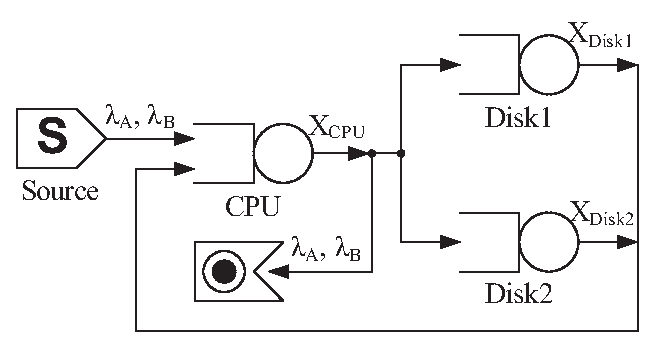
\includegraphics[scale=.65]{img/jmva/example2}
    \end{center}
    \caption{Example 2 - network topology}
    \label{fig:jmva:Example2topology}
\end{figure}
The model is characterized by two open classes $A$ and $B$ with
arrival rate (the workload intensity $\lambda$) respectively of
$\lambda_A = 0.15$ job/s and $\lambda_B=0.32$ job/s. There are three
stations of load independent type, identified with names \emph{CPU},
\emph{Disk1} and \emph{Disk2}. Service times and visits for stations
are shown in \autoref{tab:jmva:example2ServTimes} and
\autoref{tab:jmva:example2Visits}.

\begin{table}[htbp]
\begin{center}
\begin{tabular}{c|r|r|r|r|}
& \multicolumn{1}{c|}{CPU} & \multicolumn{1}{c|}{Disk1} & \multicolumn{1}{c|}{Disk2} \\
\hline
Class $A$ [s]& $0.006$ & $0.038$ & $0.030$ \\
Class $B$ [s]& $0.014$ & $0.062$ & $0.080$ \\
\hline
\end{tabular}
\end{center}
\caption{Example 2 - service times}
\label{tab:jmva:example2ServTimes}
\end{table}

\begin{table}[htbp]
\begin{center}
\begin{tabular}{c|r|r|r|r|}
& \multicolumn{1}{c|}{CPU} & \multicolumn{1}{c|}{Disk1} & \multicolumn{1}{c|}{Disk2} \\
\hline
Class $A$ & $101.0$ & $60.0$ & $40.0$ \\
Class $B$ & $44.0$ & $16.0$ & $27.0$ \\
\hline
\end{tabular}
\end{center}
\caption{Example 2 - number of visits}
\label{tab:jmva:example2Visits}
\end{table}

Since this model is similar to the network of
\autoref{fig:jmva:Example1topology} solved in
\autoref{sec:jmva:example1}, we will show how to easily create it
from a saved copy of Example~1:
\begin{enumerate*}
    \item Open the saved instance of Example~1 model
    \item Go to \texttt{Classes Tab}, change \emph{ClosedClass} name
    to \emph{A}, change its type to \texttt{Open} and set its arrival
    rate to $\lambda_A = 0.15$ job/s.
    \item Click on \emph{New Class} button, sets name of new class to
    \emph{B}, change its type to \texttt{Open} and set its arrival
    rate to $\lambda_B = 0.32$ job/s.
    \item Go to \texttt{Stations Ta}b and remove \emph{Users} delay
    center.
    \item Go to \texttt{Service Times Tab} and sets service times for
    Class $B$ according to \autoref{tab:jmva:example2ServTimes}.
    \item Go to \texttt{Visits Tab} and sets visits for
    Class $B$ according to \autoref{tab:jmva:example2Visits}.
    \item Select \texttt{Solve} action.
\end{enumerate*}

The \texttt{Synopsis Tab} with a schematic report of the model
created is shown on \autoref{fig:jmva:example2results}, while the
computed performance indices of this model are shown in
\autoref{tab:jmva:example2results}.

\begin{figure}[htbp]
    \begin{center}
        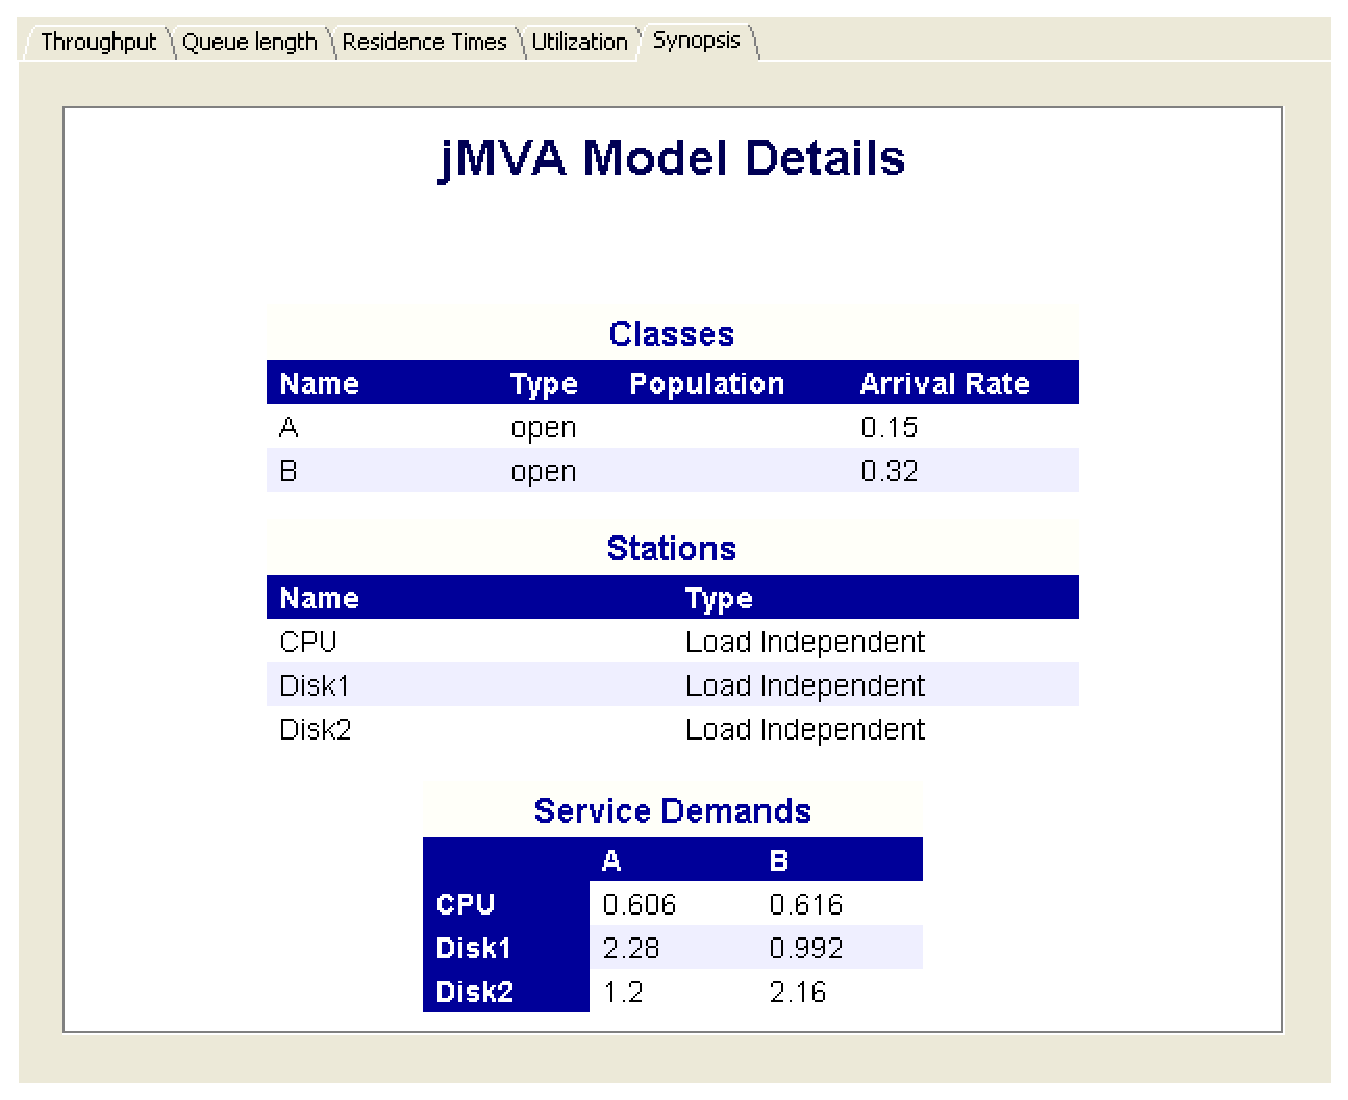
\includegraphics[scale=.5]{img/jmva/example2results}
    \end{center}
    \caption{Example 2 - output data (Synopsis Tab)}
    \label{fig:jmva:example2results}
\end{figure}

\begin{table}[htbp]
\begin{center}
\begin{tabular}{c|r|r|r|r|}
&\multicolumn{4}{c|}{Class $A$}\\
& \multicolumn{1}{c|}{Aggregate} & \multicolumn{1}{c|}{CPU} & \multicolumn{1}{c|}{Disk1} & \multicolumn{1}{c|}{Disk2}\\
\hline Throughput [job/s]& $0.150$ & $15.150$ & $9.000$ & $6.000$\\
Queue Length [job]& $2.529$ & $0.128$ & $1.004$ & $1.398$\\
Residence Time [s]& $16.863$ & $0.851$ & $6.695$ & $9.317$\\
Utilization & \multicolumn{1}{c|}{-} & $0.091$ & $0.342$ & $0.180$\\
\hline \multicolumn{5}{c}{ }\\
\multicolumn{5}{c}{ }\\
&\multicolumn{4}{c|}{Class $B$}\\
& \multicolumn{1}{c|}{Aggregate} & \multicolumn{1}{c|}{CPU} & \multicolumn{1}{c|}{Disk1} & \multicolumn{1}{c|}{Disk2}\\
\hline Throughput [job/s]& $0.320$ & $14.080$ & $5.120$ & $8.640$\\
Queue Length [job]& $6.575$ & $0.277$ & $0.932$ & $5.366$\\
Residence Time [s]& $20.548$ & $0.865$ & $2.913$ & $16.770$\\
Utilization & \multicolumn{1}{c|}{-} & $0.197$ & $0.317$ & $0.691$\\
\hline
\end{tabular}

\end{center}
\caption{Example 2 - model outputs} \label{tab:jmva:example2results}
\end{table}

\subsection{Example 3 - A model with a load dependent station}
\label{sec:jmva:example3} The network is shown in
\autoref{fig:jmva:Example3topology}.
\begin{figure}[htbp]
    \begin{center}
        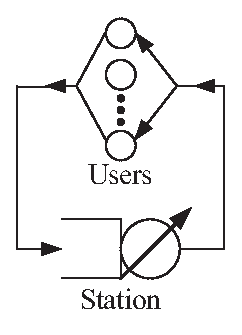
\includegraphics[scale=.65]{img/jmva/example3}
    \end{center}
    \caption{Example 3 - network topology}
    \label{fig:jmva:Example3topology}
\end{figure}
It comprises only two stations: one is of delay type (named
\emph{Users}) and the other is a load dependent station (named
\emph{Station}). This model has one closed class only with $N=8$
customers. The user's \emph{think time} is $Z = 21$ s, while the
service demands for the load dependent \emph{Station}, shown in
\autoref{tab:jmva:example3ServDemands}, are function of $n$: number
of customers in the station ($D(n) = n + 1/n$).

\begin{table}[htbp]
\begin{center}
\begin{tabular}{c|c|c|c|c|c|c|c|c|}
$n$ & $1$ & $2$ & $3$ & $4$ & $5$ & $6$ & $7$ & $8$\\
\hline
$D(n)$ [s] & $2.00$ & $2.50$ & $3.33$ & $4.25$ & $5.20$ & $6.17$ & $7.14$ & $8.13$ \\
\hline
\end{tabular}
\end{center}
\caption{Example 3 - service demands for \emph{Station}, a
load-dependent service center} \label{tab:jmva:example3ServDemands}
\end{table}

\subsubsection{Step 1 - Classes Tab}

The instructions that are the same given in Step 1 of
\autoref{sec:jmva:example1}; in this case $N$ must be 8.

\subsubsection{Step 2 - Stations Tab}

The instructions are given in Step 2 of \autoref{sec:jmva:example1};
in this case the model has two stations: a Load Dependent station
and a Delay Center.

\subsubsection{Step 3 - Service Demands Tab}

\begin{enumerate*}
\item use \texttt{Next $>$} command to switch to \texttt{Service Demands Tab}
\item double-click on cell with text \emph{LD Setting\dots}
to open the editor of load dependent service demands in a separate
window, shown in \autoref{fig:jmva:example3ldBefore}.
\item it is not mandatory to insert all values one-by-one. You can
click or drag to select cells, enter the expression $n + 1/n$ into
the textbox at the bottom of the window and click the
\emph{Evaluate} button.
\item at the end of this phase, editor window looks like
\autoref{fig:jmva:example3ldAfter}. Now you may press \emph{OK}
button to confirm changes and return to JMVA main window.
\end{enumerate*}

\begin{figure}[htbp]
    \begin{center}
        \includegraphics[scale=.5]{img/jmva/example3ldBefore}
    \end{center}
    \caption{Example 3 - editor for the description of service
    demands for a load dependent station corresponding to the different number of
    customers before the parametrization}
    \label{fig:jmva:example3ldBefore}
\end{figure}

\begin{figure}[htbp]
    \begin{center}
        \includegraphics[scale=.5]{img/jmva/example3ldAfter}
    \end{center}
    \caption{Example 3 - editor for the description of service
    demands for a load dependent station. In this case an arithmetic function
    has been defined: $S(n)=n+1/n$}
    \label{fig:jmva:example3ldAfter}
\end{figure}

\subsubsection{Step 4 - Model Resolution}

Use \texttt{Solve} command to resolve the model, results are shown
in \autoref{tab:jmva:example4results}.

\begin{table}[htbp]
\begin{center}
\begin{tabular}{c|r|r|r|r|r|}
& \multicolumn{1}{c|}{Aggregate} & \multicolumn{1}{c|}{Station} & \multicolumn{1}{c|}{Users}\\
\hline
Throughput [job/s] & $0.234$ & $0.234$ & $0.234$ \\
Queue Length [job]& $8.000$ & $3.080$ & $4.920$ \\
Residence Time [s]& $34.149$ & $13.149$ & $21.000$ \\
Utilization & \multicolumn{1}{c|}{-} & $0.810$ & $0.973$ \\
\hline
\end{tabular}
\end{center}
\caption{Example 4 - model outputs} \label{tab:jmva:example4results}
\end{table}

\subsection{Example 4 - A model with one open and one closed class}
\label{sec:jmva:example4}

The mixed queueing network model is shown in
\autoref{fig:jmva:Example4topology}.
\begin{figure}[htbp]
    \begin{center}
        \includegraphics[scale=.65]{img/jmva/example4}
    \end{center}
    \caption{Example 4 - network topology}
    \label{fig:jmva:Example4topology}
\end{figure}
Workload intensities: the open class has an arrival rate $\lambda =
1$ job/s, the closed class has a customers number $N = 57$. Service
demands are shown in \autoref{tab:jmva:example4ServDemands}.

\begin{table}[htbp]
\begin{center}
\begin{tabular}{c|r|r|r|r|}
& \multicolumn{1}{c|}{Station1} & \multicolumn{1}{c|}{Station2} & \multicolumn{1}{c|}{Station3} \\
\hline
OpenClass [s]& $0.5$ & $0.8$ & $0.6$ \\
ClosedClass [s]& $10.0$ & $4.0$ & $8.0$ \\
\hline
\end{tabular}
\end{center}
\caption{Example 4 - service demands}
\label{tab:jmva:example4ServDemands}
\end{table}

\subsubsection{Step 1 - Classes Tab}

Follow the instructions of Step~1 in the previous examples; the
\texttt{Classes Tab} is shown in \autoref{fig:jmva:example4Class}.

\begin{figure}[htbp]
    \begin{center}
        \includegraphics[scale=.5]{img/jmva/example4Class}
    \end{center}
    \caption{Example 4 - Class Tab}
    \label{fig:jmva:example4Class}
\end{figure}

\subsubsection{Step 2 - Stations Tab}

Follow the instructions of Step~2 in the previous examples; in this
case the model has three Load Independent stations (see
\autoref{fig:jmva:example4Stations}).

\begin{figure}[htbp]
    \begin{center}
        \includegraphics[scale=.5]{img/jmva/example4Stations}
    \end{center}
    \caption{Example 4 - Stations Tab}
    \label{fig:jmva:example4Stations}
\end{figure}

\subsubsection{Step 3 - Service Demands Tab}

Follow the instructions of Step~3 in the previous examples and
define service demands for both classes as illustrated in
\autoref{tab:jmva:example4ServDemands} (see
\autoref{fig:jmva:example4Services}).

\begin{figure}[htbp]
    \begin{center}
        \includegraphics[scale=.5]{img/jmva/example4Services}
    \end{center}
    \caption{Example 4 - Service Demands Tab}
    \label{fig:jmva:example4Services}
\end{figure}

\subsubsection{Step 4 - Model Solution}
Use \texttt{Solve} command. Results can be verified by computing the
\emph{equivalent model}, where the open class ``slows down'' the
closed class by subtracting utilization to it:

\begin{eqnarray*}
D_{1}^{eq}&=&\frac{D_{1,ClosedClass}}{1- \lambda * D_{1,OpenClass}} = 20 s\\
D_{2}^{eq}&=&\frac{D_{2,ClosedClass}}{1- \lambda * D_{2,OpenClass}} = 20 s\\
D_{3}^{eq}&=&\frac{D_{3,ClosedClass}}{1- \lambda * D_{3,OpenClass}} = 20 s\\
\end{eqnarray*}

MVA algorithm is used to solve the equivalent closed model. The
number of customers of the closed class is $57$, and the exact MVA
technique should require the solution of other $56$ models with
smaller population. In this particular case, the formula used to
compute the throughput can be simplified because the Service Demands
are all equals:

\begin{eqnarray*}
X^{eq}(N)&=&\frac{N}{\sum_{k=1}^{3} D_{k}^{eq} + \sum_{k=1}^{3}
\left[D_{k}^{eq}*Q_{k}^{eq}(N-1)\right]}\\
&=&\frac{N}{60 + 20*\sum_{k=1}^{3}
Q_{k}^{eq}(N-1)}\\
&=&\frac{N}{60 + 20*(N-1)}\\
\\
\\
X^{eq}(57)&=&0.048305 \textrm{ job/s}
\end{eqnarray*}

So the throughput measure for the closed class is $X_{ClosedClass} =
X^{eq} = 0.048305$ job/s while the throughput for the open class
coincide with its arrival rate $X_{OpenClass} = \lambda$. As visits
were not specified, they have been considered equal to one: that's
why throughput is equal at each station for each class (see
\autoref{fig:jmva:example4Throughput}), i.e. the solved model
consists of 3 stations that are sequentially connected with
feedback.

\begin{figure}[htbp]
    \begin{center}
        \includegraphics[scale=.5]{img/jmva/example4Throughput}
    \end{center}
    \caption{Example 4 - throughput}
    \label{fig:jmva:example4Throughput}
\end{figure}

Queue lenghts can be computed with the following formulas:
\begin{eqnarray*}
Q_{k,ClosedClass}(N)&=&Q_k^{eq}(N)\\
Q_{k,OpenClass}(N)&=&\frac{\lambda*D_{k,OpenClass}*\left[1+Q_{k,ClosedClass}(N)\right]}{1-\lambda*D_{k,OpenClass}}
\end{eqnarray*}

And the results will be equal to the ones shown in
\autoref{fig:jmva:example4Queue}.

\begin{figure}[htbp]
    \begin{center}
        \includegraphics[scale=.5]{img/jmva/example4Queue}
    \end{center}
    \caption{Example 4 - queue lengths}
    \label{fig:jmva:example4Queue}
\end{figure}

\subsection{Example 5 - Find optimal Population Mix values}
\label{sec:jmva:example5} Perform a what-if analysis to find the
value of population mix that will maximize \texttt{System
Throughput} and minimize \texttt{System Response Time} in the model
shown in \autoref{fig:jmva:Example5topology}.
\begin{figure}[htbp]
    \begin{center}
        \includegraphics[scale=.65]{img/jmva/example5}
    \end{center}
    \caption{Example 5 - network topology}
    \label{fig:jmva:Example5topology}
\end{figure}
This model has two closed classes (named \emph{Class1} and
\emph{Class2}) with a total population of $N=20$ and three load
independent stations (named \emph{Station1}, \emph{Station2} and
\emph{Station3}) with the service demands shown in
\autoref{tab:jmva:example5ServDemands}.

\begin{table}[htbp]
\begin{center}
\begin{tabular}{c|r|r|r|r|}
& \multicolumn{1}{c|}{Station1} & \multicolumn{1}{c|}{Station2} & \multicolumn{1}{c|}{Station3} \\
\hline
Class1 [s]& $1.0$ & $5.0$ & $1.0$ \\
Class2 [s]& $5.0$ & $1.0$ & $5.0$ \\
\hline
\end{tabular}
\end{center}
\caption{Example 5 - service demands}
\label{tab:jmva:example5ServDemands}
\end{table}

\subsubsection{Step 1 - Classes Tab}

Follow the instructions of Step~1 in the previous examples; as we
will change population mix, initial allocation of the $N=20$ jobs is
irrelevant. For example we can allocate $N_1=10$ jobs to
\emph{Class1} and $N_2=10$ jobs to \emph{Class2}. The
\texttt{Classes Tab} is shown in \autoref{fig:jmva:example5Class}.

\begin{figure}[htbp]
    \begin{center}
        \includegraphics[scale=.5]{img/jmva/example5Class}
    \end{center}
    \caption{Example 5 - Class Tab}
    \label{fig:jmva:example5Class}
\end{figure}

\subsubsection{Step 2 - Stations Tab}

Follow the instructions of Step~2 in the previous examples; in this
case the model has three Load Independent stations (see
\autoref{fig:jmva:example5Stations}).

\begin{figure}[htbp]
    \begin{center}
        \includegraphics[scale=.5]{img/jmva/example5Stations}
    \end{center}
    \caption{Example 5 - Stations Tab}
    \label{fig:jmva:example5Stations}
\end{figure}

\subsubsection{Step 3 - Service Demands Tab}

Follow the instructions of Step~3 in the previous examples and
define service demands for both classes as illustrated in
\autoref{tab:jmva:example5ServDemands} (see
\autoref{fig:jmva:example5Services}).

\begin{figure}[htbp]
    \begin{center}
        \includegraphics[scale=.5]{img/jmva/example5Services}
    \end{center}
    \caption{Example 5 - Service Demands Tab}
    \label{fig:jmva:example5Services}
\end{figure}

\subsubsection{Step 4 - What-if Tab}
\begin{enumerate*}
    \item use \texttt{Next $>$} command to switch to \texttt{What-if Tab}
    \item Select \texttt{Population Mix} as a \emph{control parameter} of
    the analysis in the combo box, several fields will be shown below.
    \item \emph{Class1} is already selected, by default, as reference class for the what-if
    analysis. This means that $\beta_i$ values in \texttt{From} and
    \texttt{To} fields are referred to \emph{Class1}.
    \item By default, JMVA suggests the minimum allowed value of $\beta_1$
    in the \texttt{From} field and its the maximum value in the \texttt{To}
    field\footnote{Since it is requested that one class has at least one job and customer
    number must be integer, the minimum value is $1 / N$ and the maximum value is $(N-1)/N$.}.
    Since we want to find the optimal value in the entire
    interval, we leave this unchanged.
    \item we want to perform the maximum number of allowed
    executions, so we enter a big number in the \texttt{Steps} field ($100$ for
    example). JMVA will automatically calculate the maximum number
    of allowed executions provided that number of customers for each
    class must be an integer and will report $19$.
\end{enumerate*}
At the end of this phase, the What-if Tab will look like
\autoref{fig:jmva:example5Whatif}.

\begin{figure}[htbp]
    \begin{center}
        \includegraphics[scale=.5]{img/jmva/example5Whatif}
    \end{center}
    \caption{Example 5 - What-if Tab}
    \label{fig:jmva:example5Whatif}
\end{figure}


\subsubsection{Step 5 - Model Solution}
Use \texttt{Solve} command. In the \texttt{Graphical Results Tab}
select \texttt{System Response Time} and \texttt{System Throughput}
as \emph{Performance Index}
(\autoref{fig:jmva:example5SystemResponse} and
\autoref{fig:jmva:example5SystemThroughput}). Zooming on the plot,
allows to identify the maximum value of System Throughput ($0.32$
job/s) and the minimum value of System Response Time ($62.50$ s).
They both corresponds to the execution with population mix $\beta_1
= 0.40$ for \emph{Class1}, which means that the optimal population
values are $N_1 = 8$ and $N_2 = 12$.

\begin{figure}[htbp]
    \begin{center}
        \includegraphics[scale=.5]{img/jmva/example5SystemResponse}
    \end{center}
    \caption{Example 5 - System Response Time}
    \label{fig:jmva:example5SystemResponse}
\end{figure}

\begin{figure}[htbp]
    \begin{center}
        \includegraphics[scale=.5]{img/jmva/example5SystemThroughput}
    \end{center}
    \caption{Example 5 - System Throughput}
    \label{fig:jmva:example5SystemThroughput}
\end{figure}

%
% This document is free; you can redistribute it and/or modify
% it under the terms of the GNU General Public License as published by
% the Free Software Foundation; either version 2 of the License, or
% (at your option) any later version.
%
% This document is distributed in the hope that it will be useful, but
% WITHOUT ANY WARRANTY; without even the implied warranty of
% MERCHANTABILITY or FITNESS FOR A PARTICULAR PURPOSE.  See the GNU
% General Public License for more details.
%
% You should have received a copy of the GNU General Public License
% along with this document; if not, write to the Free Software
% Foundation, Inc., 51 Franklin Street, Fifth Floor, Boston, MA
% 02110-1301, USA.
%
% Author: Bertoli Marco
%
\chapter{JSIM}
\label{cha:jsim}
\section{Overview}
JSIM analyzes open, closed and mixed queueing networks using a discrete-event simulator \cite{DESimulation}. A sequence of \emph{wizard} windows helps specifying network properties. The simulation engine supports several probability distributions for characterizing service and inter-arrival times, e.g., exponential, hyperexponential, uniform, Erlang and Pareto. Random number generation is based on the Mersenne twister engine \cite{Mersenne}. It is also possible to reproduce a given sequence of random numbers, in order to simulate real workloads from collected
log files. Load-dependent strategies using arbitrary functions of the current queue-length can be specified.

JSIM supports state-independent routing strategies, e.g., Markovian or round robin, as well as state-dependent strategies, e.g., routing to the server with minimum utilization, or
with the shortest response time, or with minimum queue length.

Performance indices like throughputs, utilizations, response times, residence times, queue-lengths are evaluated. The simulation engine supports several extended features
not allowed in product-form models, namely, finite capacity regions (i.e., blocking), fork-join servers, and priority classes. Finite capacity regions may include either shared
or class-specific population constraints. 

The analysis of simulation results employs on-line transient detection techniques based on spectral analysis \cite{Spectral}. What-if analysis, where a sequence of simulations is run for different
values of parameters, are also possible.

\subsection{Starting the alphanumeric simulator}
Selecting \includegraphics[scale=.5]{img/JSIMIcon} button on the
starting screen, \autoref{fig:jsim:Classes} window shows up.
\begin{figure}[htb]
    \begin{center}
        \includegraphics[width=300pt]{img/jsim/classes}
    \end{center}
    \caption{Classes Panel}
    \label{fig:jsim:Classes}
\end{figure}
Each JSIM panel is organized to be compliant with a given layout, shown in \autoref{fig:jsim:panellayout}, 
\begin{figure}[tb]
    \begin{center}
        \includegraphics[width=300pt]{img/jsim/panelLayout}
    \end{center}
    \caption{Layout of JSIM panels}
    \label{fig:jsim:panellayout}
\end{figure}
where the following main areas can be identified:


\appendix
%
% This document is free; you can redistribute it and/or modify
% it under the terms of the GNU General Public License as published by
% the Free Software Foundation; either version 2 of the License, or
% (at your option) any later version.
%
% This document is distributed in the hope that it will be useful, but
% WITHOUT ANY WARRANTY; without even the implied warranty of
% MERCHANTABILITY or FITNESS FOR A PARTICULAR PURPOSE.  See the GNU
% General Public License for more details.
%
% You should have received a copy of the GNU General Public License
% along with this document; if not, write to the Free Software
% Foundation, Inc., 51 Franklin Street, Fifth Floor, Boston, MA
% 02110-1301, USA.
%
% Author: Bertoli Marco
%
\chapter{Basic Definitions}
\label{cha:glossary}
\begin{description}
\item[Customer :] or \emph{job} or \emph{transaction} is the element that will require
service from our network. For example, it can be an \emph{http
request}, a \emph{database query}, or an \emph{ftp download
command}.
\item[Class :] a group of elements that are statistically equal.
The customers of a class have the same workload intensity and the
same average service demands.
\item[Station :] or service center, it represents a system resource.
Customers arrive at the station and then, if necessary, wait in
queue, receive service from server then depart.
\item[Bottleneck Station :] a station with the highest utilization
\item[Potential Bottleneck Station :] a station that can become bottleneck for some feasible network population
\item[Dominated Stations :] a station P is dominated if exist al least a station Q whose demand for each classes of custumer are highest or equal (but at least one highest) than those of P.
\item[Masked-off Stations :] a station that is not a Potential Bottleneck or a Dominated station.A Masked-off station may exhibit the largest queue-lungth and hence the highest response time.
\item[Workload Intensity ($\lambda$ or $N$) :] rate at which customers of a
given class arrive at the system.  Each class has its own workload
intensity. If a class is closed the constant \emph{number of
customers} $N$ that are present in the system must be provided, if a
class is open the \emph{arrival rate} $\lambda$ of customers to the
system is requested.
\item[Population Mix ($\beta_i$) :] the ratio between \emph{number of
customers} of closed class $i$ and the total number of customers in
the system: $\beta_i = N_i / \sum_k N_k$
\item[Saturarion Sector :] a interval of Population Mix in witch one, two ore more stations are both bottleneck.
\item[Service Time ($S_k$):] average time of service required at
each visit to resource $k$; it is computed as the ratio of the busy
time to the number of system completions. It is an alternatively way
to describe the service requirement.
\item[Visit (number of -) ($V_k$) :] average number of visits that
a customer makes at station $k$ during a complete execution; it is
computed as the ratio of the number of completions at resource k to
the number of system completions. If resource $k$ is a delay center
representing a client station, it is a convention assign a unitary
value to number of visits to this station.
\item[Service Demand ($D_k$) :] average service requirement of
a customer, that is the total amount of service required  by a
complete execution at resource $k$. In the model it is necessary to
provide separate service demand for each pair service center-class.
It is given by $D_k = V_k * S_k$.
\item[Throughput ($X_k$) :] rate at which customers are executed
by station $k$, that is the number of completions in a time unit.
\item[Queue length ($Q_k$) :] average number of customers at station
$k$, either waiting in queue and receiving service.
\item[Response Time ($R_k$):] average time interval between the instant
a customer arrives at station $k$ and the instants it terminate its
servicing.
\item[Residence Time ($W_k$) :] average
time that a customer spent at station $k$ during a complete
interaction with the system. It includes time spent queueing and
time spent receiving service. It does not correspond to
\emph{Response Time} $R_k$ of a station since $W_k = R_k * V_k$.
\item[Utilization ($U_k$) :] proportion of time in which the station $k$ is busy or, in the case
of a delay center, is the average  number of  customers in the
station (see Little Law \cite{Little}).
\item[System Throughput ($X$) :] rate at which customers perform
an entire interaction with the system. This is the aggregate measure
of \emph{Throughput}: $X = X_k / V_k$.
\item[System Response Time ($R$):] correspond to the intuitive
notion of response time perceived by users, that is, the time
interval between the instant of the submission of a request to a
system and the instant the corresponding reply arrives completely at
the user. It is the aggregate measure of \emph{Residence Times}: $R
= \sum_k W_k$.
\item[Average number of customers in the system ($N$):] the average
number of customer in the system, either waiting in queue or
receiving service. It is the aggregate measure of \emph{Queue
Length}: $N = \sum_k Q_k$.
\end{description}


\bibliographystyle{alpha}
\linespread{1}
\bibliography{manual}

\end{document}
